%&preambule
%\input{preambule}

%----- géométrie des pdf
% \geometry{a4paper, landscape} % format paysage
% \geometry{a5paper, left=1cm, right=1cm, top=0.8cm, bottom=2cm} % format A5
% \geometry{a5paper, left=1cm, right=1cm, top=2cm, bottom=2cm} % format A5 avec en-tête

%----- en-tête et mode correction
% \modeCorrection % correction (décommenté)
\renewcommand{\etablissement}{Lycée Jean Moulin} % pour l'en-tête

%------ doc
\begin{document}
  %------ Matériel de TP
  %% Titre de la fiche de TP
\newcommand{\titreFicheTP}[1]{
  \newpage
  \begin{boiteColoree}[couleurPrim]
    \centering
    \important[white]{\Large Fiche de préparation de TP}
  
    \important[white]{#1}
  \end{boiteColoree}
}

%% Tableau de préambule 
% \preambuleFicheTP{classe}{horaire dans l'emploi du temps}
\NewDocumentCommand{\preambuleFicheTP}{m +m}{
  \begin{center}
    \begin{tblr}{
        colspec = {l X[c] l X[c] l X[c]},
        width = \linewidth, column{1,3,5} = {couleurPrim-100},
      }
      \important{Prof :}    & Alexandre Jedrecy &
      \important{Matière :} & Physique-Chimie &
      \important{Niveau :}  & #1 \\
    \end{tblr}

    \begin{tikzpicture}
      \emploiDuTemps[hauteur jours = 0.8cm]
      #2
    \end{tikzpicture}
  \end{center}
}

%% Préambule seconde
% \ficheSecondeTP {titre} {date}
\newcommand{\ficheSecondeTP}[1]{
  \titreFicheTP{#1}
  \preambuleFicheTP{Seconde}{
    \evenement[creneau = 8, titre = 2GT2-1, lieu = A108]
    \evenement[creneau = 6, titre = 2GT4-2, jour = 2, lieu = A108];
    \evenement[creneau = 1, titre = 2GT4-1, jour = 5];
    \evenement[creneau = 6, titre = 2GT2-2, jour = 5];
  }
}
\newcommand{\effectifSeconde}{
  \begin{multicols}{2}
    \important{Effectif :} 15
  
    \flecheLongue \important{7 groupes} de 2 élèves
  \end{multicols}
  \vspace*{-12pt}
}

%% Préambule première ST2S
% \fichePremiereStssTP {titre} {date}
\newcommand{\fichePremiereStssTP}[1]{
  \titreFicheTP{#1}
  \preambuleFicheTP{Première ST2S}{
    \evenement[creneau = 2, titre = 1ST2S1-1, lieu = A103, couleur = purple-200]
    \evenement[creneau = 6, titre = 1ST2S1-2, lieu = A108, couleur = purple-200]
  }
}
\newcommand{\effectifPremiereStss}{
  \begin{multicols}{2}
    \important{Effectif :} 12
    
    \flecheLongue \important{6 groupes} de 2 élèves
  \end{multicols}
  \vspace*{-12pt}
}

%% Préambule terminale ST2S
% \ficheTerminaleStssTP {titre} {date}
\newcommand{\ficheTerminaleStssTP}[1]{
  \titreFicheTP{#1}
  \preambuleFicheTP{Terminale ST2S}{
    \evenement[creneau = 8, titre = TST2S1-1, jour = 2, couleur = red-200]
    \evenement[creneau = 3, titre = TST2S1-2, jour = 3, lieu = A103, couleur = red-200]
  }
}
\newcommand{\effectifTerminaleStss}{
  \begin{multicols}{2}
    \important{Effectif :} 12
    
    \flecheLongue \important{6 groupes} de 2 élèves
  \end{multicols}
  \vspace*{-12pt}
}
  %--- Seconde
% \input{fichesTP/seconde/TP_cocktail_vinaigrette}
% \ficheSecondeTP{Répression des fraudes}

\begin{boiteMateriel}{Matériel élève}
  \effectifSeconde
  
  \begin{protocole}[2]
    \item 1 pipette jaugée de 10 mL.
    \item 1 poire de prélèvement.
    \item 1 éprouvette graduée de 50 mL.
    \item 2 béchers de 50 mL.
    \item 1 balance précises à 0,1 g.
    \item[\vspace{\fill}]
  \end{protocole}
\end{boiteMateriel}


\begin{boiteMateriel}{À préparer}
  \begin{protocole}
    \item 1 solution de 500 mL d'éthanol à 70 $\%$ (ou tout autre $\%$ si tu en as un autre déjà prêt).
    \item 2 bécher de 500 mL (ou 250 mL).
    \item 1 bouteille de sirop.
  \end{protocole}
\end{boiteMateriel}
\ficheSecondeTP{Identifier des solides et des liquides}

\begin{boiteMateriel}{Matériel élève}
  \effectifSeconde
  
  \begin{protocole}[2]
    \item 1 éprouvette graduée de 50 mL
    \item 4 tubes à essais
    \item 1 balance
    \item 1 set de cylindres métalliques
    %\item [\vspace{\fill}]
  \end{protocole}
\end{boiteMateriel}


\begin{boiteMateriel}{À préparer}
  \vspace*{4pt}
  \begin{protocole}[2]
    % \item 2 plaques de cuivre
    % \item 2 plaques d'aluminium
    % \item 2 plaques de zinc
    % \item 2 plaques de fer
    \item 3 béchers de 200 mL
    \item 1 bouteille de Cristalline, Mont Roucous et Vichy St Yorre
    \item nitrate d'argent
    \item chlorure de baryum
    \item oxalate d'ammonium
    \item hydroxyde de sodium
    %\item [\vspace{\fill}]
  \end{protocole}
\end{boiteMateriel}
% \ficheSecondeTP{Séparer et identifier des espèces chimiques}

\begin{boiteMateriel}{Matériel élève}
  \effectifSeconde
  
  \begin{protocole}[2]
    \item 1 cuve CCM %avec $\sim \qty{1}{\cm}$ d'éluant (alcool à 50 \%)
    \item 1 plaque à CCM
  \end{protocole}
\end{boiteMateriel}


\begin{boiteMateriel}{À préparer}
  \begin{protocole}
    \item 1 pissette d'eau distillée
    \item 6 coupelles de pesée en verre
    \item 1 paquet de cures-dents
    \item 1 paquet de M\&M's
    \item Des colorants alimentaires
    \item 200 mL d'alcool à \qty{50}{\percent}
  \end{protocole}
\end{boiteMateriel}
% \ficheSecondeTP{Dosage par étalonnage}

\begin{boiteMateriel}{Matériel élève}
  \effectifSeconde

  \begin{protocole}[2]
    \item 1 sabot de pesée
    \item 1 fiole jaugée de 50 mL
    \item 1 bécher de 100 mL
    \item 1 pipette pasteur
    \item 1 pissette d’eau du robinet
    \item [\vspace{\fill}]
  \end{protocole}
\end{boiteMateriel}


\begin{boiteMateriel}{À préparer}
  \vspace*{4pt}
  \begin{protocole}[2]
    \item 1 bouteille de sirop
    \item 2 pipette jaugée de 10 mL
    \item 1 bêcher 50 mL
    \item 1 bêcher 100 mL
    \item 1 paquet de sucre
    \item 1 pissette d’eau
    \item 2 balances
    \item [\vspace{\fill}]
  \end{protocole}
\end{boiteMateriel}
% \ficheSecondeTP{Dosage d'un produit désinfectant}

\begin{boiteMateriel}{Matériel élève}
  \effectifSeconde

  \begin{protocole}
    \item 1 pipette graduée de 10 mL.
    \item 1 fiole jaugée de 25 mL.
    \item 1 bouchon adapté à la fiole jaugée.
    \item 4 bécher de 50 mL.
    \item 1 support à tube à essais avec 4 tubes à essais.
    \item 1 pissette d'eau (du robinet).
  \end{protocole}
\end{boiteMateriel}


\begin{boiteMateriel}{À préparer}
  \begin{protocole}
    \item 1 solution de permanganate de potassium.
    \item 1 bécher de 100 mL.
    \item 1 bécher de 250 mL.
    \item des gants de protection.
    \item du Dakin.
  \end{protocole}
\end{boiteMateriel}
% \input{fichesTP/seconde/TP_formation_images}
% \input{fichesTP/seconde/TP_refraction_lumiere}
% \ficheSecondeTP{Dénombrer un grand nombre d’entités identiques}

\begin{boiteMateriel}{Matériel élève}
  \effectifSeconde

  \begin{protocole}
    \item 2 béchers de 100 mL.
  \end{protocole}
\end{boiteMateriel}


\begin{boiteMateriel}{À préparer}
  \begin{protocole}
    \item 1 spatule.
    \item 1 sachet de riz de 1 kg.
    \item 2 balances précise à 0,1 g + alimentation adaptée.
  \end{protocole}
\end{boiteMateriel}
% \ficheSecondeTP{Extincteur chimique}

\begin{boiteMateriel}{Matériel élève}
  \effectifSeconde
  
  \begin{protocole}[2]
    \item 1 fiole jaugée de 50 mL
    \item 1 éprouvette graduée de 50 mL
    \item 1 bécher de 50 mL
    \item 1 sabot de pesée
  \end{protocole}
\end{boiteMateriel}


\begin{boiteMateriel}{À préparer}
  \begin{protocole}
    \item 1 sac de ballons gonflables
    \item 1 sachet de bicarbonate de soude
    \item 1 bouteille de vinaigre blanc
    \item 2 balances
    \item 2 spatules
  \end{protocole}
\end{boiteMateriel}

% \ficheSecondeTP{Se chauffer au gaz}

\begin{boiteMateriel}{Matériel élève}
  \effectifSeconde
  
  \begin{protocole}[2]
    \item 2 bécher de 50 mL
    \item 1 thermomètre
    \item 1 ExAO
    \item 1 pissette d'eau distillée
    \item 1 sabot de pesée
  \end{protocole}
\end{boiteMateriel}


\begin{boiteMateriel}{À préparer}
  \begin{protocole}
    \item 2 balances
    \item 2 spatules
    \item 1 sachet de sel
    \item 1 bidon de pastilles d'hydroxyde de sodium
  \end{protocole}
\end{boiteMateriel}

% \input{fichesTP/seconde/TP_loi_ohm}

%--- Première ST2S
% \input{fichesTP/stssPremiere/TP_dilution_desinfectant}
% \input{fichesTP/stssPremiere/TP_pH_acide_base}
% \input{fichesTP/stssPremiere/TP_formation_image}
% \input{fichesTP/stssPremiere/TP_test_fehling}

%--- Terminale ST2S
% \ficheTerminaleStssTP{Fraîcheur d'un lait}

\begin{boiteMateriel}{Matériel élève}
  \effectifTerminaleStss

  \begin{listePoints}
    \item 1 burette et son support.
    \item 1 agitateur magnétique.
    \item 1 barreau aimanté.
    \item 1 erlen-meyer 250 mL.
    \item 2 bécher 100 mL.
    \item 1 éprouvette graduée 50 mL.
  \end{listePoints}
\end{boiteMateriel}

\begin{boiteMateriel}{À préparer}
  \begin{listePoints}
    \item 500 mL de solution d'hydroxyde de sodium $c = \qty{0,05}{\mol\per\litre}$.
    \item 1 bouteille de lait > 0,5 L.
    \item 1 solution de bleu de bromothymol.
  \end{listePoints}
\end{boiteMateriel}
% \ficheTerminaleStssTP{Réalisation pratique d'une échographie}

\begin{boiteMateriel}{Matériel élève}
  \effectifTerminaleStss

  \begin{listePoints}[2]
    \item 1 couple émetteur/récepteur ultrasonore
    \item 1 oscilloscope.
    \item 1 générateur 12 V.
    \item 1 câble BNC/banane.
    \item 2 câble banane rouge et noir.
  \end{listePoints}
  %Note : de mémoire il n'y a que trois câble BNC/banane, mais si il y a de quoi faire 5 groupes je suis preneur.
\end{boiteMateriel}

\begin{boiteMateriel}{À préparer}
  \begin{listePoints}
    \item 1 ensemble d'échantillons de matériaux.
    \item 1 gel pour échographie.
  \end{listePoints}
  Les deux se trouvent dans le même placard que les émetteurs/récepteur à ultrason de mémoire.
\end{boiteMateriel}
% \ficheTerminaleStssTP{Combustion d'une bougie}

% \begin{boiteMateriel}{Matériel élève}
%   \effectifTerminaleStss
% \end{boiteMateriel}

\begin{boiteMateriel}{À préparer}
  \begin{listePoints}
    \item Un cristallisoir.
    \item Deux bougies.
    \item Une boite d’allumettes ou un briquet.
    \item Une éprouvette graduée de 500 mL.
  \end{listePoints}
\end{boiteMateriel}


  %------ Cours et activités
  %% Méthodes
% %%%%
\teteSndMeth

%%%% titre
\vspace*{-36pt}
\numeroActivite{1}
\titreActivite{Notation scientifique et unités}

% \begin{objectifs}
%   \item Revoir les puissances de 10 et la notation scientifique
% \end{objectifs}

%%%%
\vspace*{-20pt}
\titreSection{Rappels sur les puissance de 10}
\vspace*{-8pt}

%%
\begin{doc}{Les puissances de 10}{doc:A1_puissance_10}
  Les puissances indiquent qu'on va répéter une multiplication ($2^3 = 2 \times 2 \times 2 = 8$).
  
  Pour lire les puissances de 10, il suffit de suivre deux règles simple
  \begin{importants}
    \pointCyan Écrire le nombre $10^a$ (avec $a = 0, 1, 2, 3, \ldots$), revient à écrire ``$1$'' suivi de $a = 0, 1, 2, 3, \ldots$ zéros. \\
    \exemple \num{e3} = \texteTrou[0.2]{\num{1000}}

    \pointCyan Écrire le nombre $10^{-a}$ (avec $a = 1, 2, 3, \ldots$), revient à écrire ``$0,$'' suivi de $a - 1 = 0, 1, 2, \ldots$ zéros et d'un $1$. \\
    \exemple \num{e-2} = \texteTrou[0.2]{\num{0,01}}
  \end{importants}
\end{doc}


\numeroQuestion Écrire les nombres correspondant aux puissances de 10 suivantes : \\
$\num{e2}  =$ \texteTrou[0.1]{\num{100}} \qq{}
$\num{e5}  =$ \texteTrou[0.1]{\num{100000}} \qq{}
$\num{e-3} =$ \texteTrou[0.1]{\num{0,001}} \qq{}
$\num{e-1} =$ \texteTrou[0.1]{\num{0,1}}

\numeroQuestion Écrire les nombres suivants comme le produit d'un nombre compris entre 0 et 9 et d'une puissance de 10 \exemple \num{600} = \num{6,00e2} :
\pasCorrection{\vspace*{-4pt}}
\begin{listePoints}[2]
  \setlength\itemsep{-4pt}
  \item \num{100000}  = \texteTrouLignes{\num{1e5}}
  \item \num{1}       = \texteTrouLignes{\num{1e0}}
  \item \num{9000000} = \texteTrouLignes{\num{9e6}}
  \item \num{0,1}     = \texteTrouLignes{\num{1e-1}}
  \item \num{0,0006}  = \texteTrouLignes{\num{1e-4}}
  \item \num{0,00705} = \texteTrouLignes{\num{7,05e-3}}
\end{listePoints}


%%
\pasCorrection{\vspace*{-26pt}}
\begin{doc}{Règles de calculs}{doc:A1_calcul_puissance_10}
  Il y a deux règles de calculs à connaître pour les puissances de 10
  \begin{importants}
    \pointCyan $10^a \times 10^b = 10^{a + b}$ \\   
    \pointCyan $10^{-a} = \dfrac{1}{10^a}$
  \end{importants}
\end{doc}


\numeroQuestion Réaliser les calculs suivants :
\pasCorrection{\vspace*{-4pt}}
\begin{listePoints}[2]
  \setlength\itemsep{-4pt}
  \item $10^2 \times 10^1 =$ \texteTrouLignes{$10^{2 + 1} = 10^3 = 1000$}
  \item $10^4 \times 10^{-3} =$ \texteTrouLignes{$10^{4 - 3} = 10^1 = 10$}
  \item $10^{-2} \times 10^{-3} =$ \texteTrouLignes{$10^{-2 - 3} = 10^{-5} = 0,00001$}
  \item $10^{-1} \times 10^{-5} \times 10^4 =$ \texteTrouLignes{$10^{-1 - 5 + 4} = 10^{-2} = 0,01$}
\end{listePoints}


%%
\pasCorrection{\vspace*{-26pt}}
\begin{doc}{Moyen mnémotechnique}{doc:A1_decalage_virgule}
  \begin{listePoints}
    \setlength\itemsep{-4pt}
    \item Si je décale la virgule de 1 rang vers la gauche, alors
    \texteTrou[0.25]{je réduis} de 1 unité la puissance de dix. \texteTrou{J'ai divisé par 10.}
    \item Si je décale la virgule de 1 rang vers la droite, alors
    \texteTrou[0.35]{j'augmente} de 1 unité la puissance de dix. \texteTrou{J'ai multiplié par 10.}
  \end{listePoints}
\end{doc}


%%%%
\newpage
\vspace*{-36pt}
\titreSection{Notation scientifique}

\vspace*{-12pt}
\begin{doc}{La notation scientifique}{doc:A1_notation_scientifique}
  \begin{importants}
  La \important{notation scientifique} d'une quantité se présente de la façon suivante :
  % Textes
  \begin{center}
    \texteEncadre{chiffre différent de zéro}
    \hspace{5pt}
    \texteEncadre{autres chiffres} 
    \qq{}
    \texteEncadre{puissance de dix}
    \texteEncadre{\important{unité}}
  \end{center}
  % Virgule et multiplication
  \vspace*{-32pt}
  \begin{tikzpicture}  
    \draw [white] (0,0) circle;
    \draw [couleurSec, thick] (5.6,-0.4) circle [radius=0.3] node {$,$};
    \draw [couleurSec, thick] (9.5,0.0) circle [radius=0.3] node {$\times$};
  \end{tikzpicture}
  \end{importants}
\end{doc}

\numeroQuestion Écrire les quantités suivantes en notation scientifique :
\vspace*{-8pt}
\begin{listePoints}[2]
  \item \qty{288}{\hour}      = \texteTrouLignes{\qty{2,88e2}{\hour}\\}
  \item \qty{1}{\m}           = \texteTrouLignes{\qty{1e0}{\m}\\}
  \item \qty{756 864 000}{\s} = \texteTrouLignes{\qty{7,56 864 000}{8\s}\\}
  \item \qty{638}{\newton}    = \texteTrouLignes{\qty{6,38e2}{\newton}}
  \item \qty{0,01}{\percent}  = \texteTrouLignes{\qty{1,0e-2}{\percent}\\}
  \item \qty{8960}{\g/\l}     = \texteTrouLignes{\qty{8,96e3}{\g/\l}\\}
  \item \qty{0,436}{\s}       = \texteTrouLignes{\qty{4,36e-1}{\s}\\}
  \item \qty{0,336}{\s}       = \texteTrouLignes{\qty{3,36e-1}{\s}}
\end{listePoints}
\vspace*{-16pt}

\attention Il faut \important{toujours} préciser \important{l'unité} d'une grandeur quand on réalise un calcul !
Les grandeurs sans unités sont rares en physique-chimie.


%%%%
\titreSection{Le système international de mesure}

%%
\vspace*{-12pt}
\begin{doc}{Le système international}{doc:A1_SI}
  Pour comparer des grandeurs entre elles, il faut les exprimer avec les \important{mêmes unités de mesures.} % exemple centime et euros
  
  Pour pouvoir communiquer facilement d'un pays à un autre, le \important{système international (SI)} a été développé par la Conférence Générale des Poids et Mesures (CGPM).
  Le système international est composé de \important{sept unités de bases.}

  En physique on est amené à décrire des \important{échelles} très variées, par exemple quand on mesure la taille d'un cheveu ($\sim \qty{e-6}{\metre}$) ou la taille d'une planète ($\sim \qty{e7}{\metre})$.
  
  \begin{importants}
    Pour simplifier la manipulation des grandeurs éloignées de l'unité, chaque \important{puissance de \num{1000}} est associée à un \important{préfixe} dans le système international.
  \end{importants}

  \begin{center}
    \begin{tblr}{
      hlines, vlines, row{1} = {couleurPrim!20}, colspec = {c c c l}
    }
      Puissance  & Préfixe & Symbole & Nombre décimal \\
      \num{e12}  & tera    & T       & \num{1 000 000 000 000} \\
      \num{e9}   & giga    & G       & \num{1 000 000 000} \\
      \num{e6}   & mega    & M       & \num{1 000 000} \\
      \num{e3}   & kilo    & k       & \num{1 000} \\
      $10^0$     &         &         & \num{1} \\
      \num{e-3}  & milli   & m       & \num{0,001} \\
      \num{e-6}  & micro   & $\mu$   & \num{0,000 001} \\
      \num{e-9}  & nano    & n       & \num{0,000 000 001} \\
      \num{e-12} & femto   & f       & \num{0,000 000 000 001}
    \end{tblr}
  \end{center}
\end{doc}
 % début 1h
% %%%%
\teteSndMeth

%%%% titre
\vspace*{-36pt}
\numeroActivite{1}
\titreTP{Découverte du laboratoire}


%%%% objectifs
\begin{objectifs}
  \item Connaître les pictogrammes de sécurité
  \item Connaître la verrerie de base en chimie
\end{objectifs}


%%%% docs
\begin{doc}{Les pictogrammes de sécurités}{doc:TP0_picto_secu}
  Les pictogrammes de sécurités sont à connaître par c\oe{}ur ! \\[4pt]

  %% Tableau avec les pictogrammes
  \NewDocumentCommand{\pictoTableau}{m O{65}}{
    \hspace{16pt} \image{0.45}{images/securite/picto_#1} \vAligne{-#2pt}
  }
  \begin{tblr}{
    colspec = {|X[-1, h, m] | X[4, m] |}, hlines,
    row{1} = {couleurPrim!20, c}
  }
    \textbf{Pictogramme} & \textbf{Signification} \\
    %
    \pictoTableau{corrosif} &
    {\texteTrou{Corrosif.} \\
    Je peux attaquer ou détruire les métaux.
    Je ronge la peau et/ou les yeux en cas de contact.} \\
    %
    \pictoTableau{nocif} &
    {\texteTrou{Toxique, irritant, narcotique.} \\
    J'empoisonne à forte dose.
    J'irrite la peau, les yeux et/ou les voies respiratoires.
    Je peux provoquer des allergies, de la somnolence ou des vertiges.} \\
    %
    \pictoTableau{toxique}[55] &
    {\texteTrou{Toxique.} \\
    J’empoisonne rapidement, même à faible dose.} \\
    %
    \pictoTableau{explosif} &
    {\texteTrou{Explosif.} \\
    Je peux exploser au contact d’une flamme, d’une étincelle, d’électricité statique, sous l’effet de la chaleur, de frottements ou d’un choc.} \\
    %
    \pictoTableau{combustible} &
    {\texteTrou{Inflammable.} \\
    Je peux m’enflammer au contact d’une flamme, d’une étincelle, d’électricité statique, sous l’effet de la chaleur, de frottements ou au contact de l’air ou de l’eau.} \\
    %
    \pictoTableau{comburant} &
    {\texteTrou{Comburant.} \\
    Je peux provoquer ou aggraver un incendie ou même provoquer une explosion en présence de produits inflammables.} \\
    %
    \pictoTableau{gaz_pression} &
    {\texteTrou{Gaz sous pression.} \\
    Je peux exploser sous l’effet de la chaleur.
    Je peux causer des brûlures ou blessures liées au froid.} \\
    %
    \pictoTableau{environnement} &
    {\texteTrou{Dangereux pour l'environnement.} \\
    Je provoque des effets néfastes sur les organismes du milieu aquatique, sur les êtres vivants.} \\
    %
    \pictoTableau{reprotoxique} &
    {\texteTrou{Mutagène, cancerogène, reprotoxique.} \\
    Je peux provoquer le cancer, modifier l’ADN, nuire à la fertilité ou au f\oe{}tus, altérer le fonctionnement des organes.
    Je peux être mortel en cas d’ingestion dans les voies respiratoires.}
    %
  \end{tblr}
\end{doc}

%%
\begin{doc}{Verrerie}{doc:TP0_verrerie}
  \begin{importants}
    La \important{verrerie} désigne l'ensemble des contenants utilisés pour réaliser des manipulations en chimie.
  \end{importants}
  La majorité de ces contenants sont en verre, c'est pour ça qu'on parle de \textit{verre}rie.
\end{doc}


%%
\numeroQuestion Associer à chaque schéma de verrerie son nom.

\begin{multicols}{4}
  \centering
  \image{1}{images/chimie/verrerie/schema0001} \\[-18pt]
  \pointCyan \\[3cm]
  \pointCyan \\ Bécher

  \image{1}{images/chimie/verrerie/schema0002} \\[-18pt]
  \pointCyan \\[3cm]
  \pointCyan \\ Coupelle de pesée
  
  \image{1}{images/chimie/verrerie/schema0003} \\[-18pt]
  \pointCyan \\[3cm]
  \pointCyan \\ Ballon monocol
  
  \image{1}{images/chimie/verrerie/schema0004} \\[-18pt]
  \pointCyan \\[3cm]
  \pointCyan \\ Éprouvette graduée
\end{multicols}
\vspace*{1cm}

\begin{multicols}{4}
  \centering
  \image{1}{images/chimie/verrerie/schema0005} \\[-6pt]
  \pointCyan \\[3cm]
  \pointCyan \\ Poire
  
  \image{1}{images/chimie/verrerie/schema0006} \\[-6pt]
  \pointCyan \\[3cm]
  \pointCyan \\ Verre à pied
  
  \image{1}{images/chimie/verrerie/schema0007} \\[-6pt]
  \pointCyan \\[3cm]
  \pointCyan \\ Erlenmeyer 
  
  \image{1}{images/chimie/verrerie/schema0008} \\[-6pt]
  \pointCyan \\[3cm]
  \pointCyan \\ Pipette jaugée
\end{multicols} % début 1h
% \input{seconde/A2_analyse_dimensionnelle} % début mécanique 1h
% %%%%
\teteSndMeth

%%%% titre
\numeroActivite{3}
\titreActivite{Ordre de grandeur}


%%%%
\vspace*{-24pt}
\titreSection{Notation scientifique}

%%
\begin{doc}{Les puissances de 10}{doc:A1_puissance_10}
  \begin{encart}
  \begin{listePoints}
    \item Écrire le nombre $10^n$ (avec $n = 0, 1, 2, 3, \ldots$), revient à écrire ``$1$'' suivi de $n = 0, 1, 2, 3, \ldots$ zéros. \textit{Exemple : $10^3 = 1000$}
    \item Écrire le nombre $10^{-n}$ (avec $n = 1, 2, 3, \ldots$), revient à écrire ``$0,$'' suivi de $n - 1 = 0, 1, 2, \ldots$ zéros et d'un $1$. \textit{Exemple : $10^{-2} = 0,\!01$}
    \item $10^a \times 10^b = 10^{a + b}$
    \item $\dfrac{1}{10^n} 
    = \dfrac{10^{-n}}{10^{-n}} \times \frac{1}{10^n} 
    = \dfrac{10^{-n}}{10^{n - n}}
    = \dfrac{10^{-n}}{10^0}
    = 10^{-n}$
  \end{listePoints}
  \end{encart}
\end{doc}
\bigskip

\begin{doc}{Moyen mnémotechnique}{doc:A1_decalage_virgule}
  \begin{listePoints}
    \item Si je décale la virgule de 1 rang vers la gauche, alors \texteTrouLignes{je réduis de 1 unité} la puissance de dix.
    \item Si je décale la virgule de 1 rang vers la droite, alors \texteTrouLignes{j'augmente de 1 unité}
    la puissance de dix.
  \end{listePoints}
\end{doc}

\begin{doc}{La notation scientifique}{doc:A1_notation_scientifique}
  \begin{encart}
  La \important{notation scientifique} d'une quantité se présente de la façon suivante :
  % Textes
  \begin{center}
    \texteEncadre{chiffre différent de zéro}
    \qq{}
    \texteEncadre{autres chiffres} 
    \qq{}
    \texteEncadre{puissance de dix}
    \texteEncadre{\important{unité}}
  \end{center}
  % Virgule et multiplication
  \vspace*{-30pt} \hspace*{4pt}
  \begin{tikzpicture}  
    \draw [white] (0,0) circle;
    \draw [couleurSec, thick] (5.5,-0.25) circle [radius=0.3] node {$,$};
    \draw [couleurSec, thick] (9.65,0) circle [radius=0.3] node {$\times$};
  \end{tikzpicture}
  \end{encart}
\end{doc}

\numeroQuestion Écrire les quantités suivantes en notation scientifique :
  
\separationBlocs{
  \qty{288}{\hour}       = \texteTrouLignes{\qty{2,88e2}{\hour}}
  \qty{756864000}{\s} = \texteTrouLignes{\qty{7,56864}{\s}}
}{
  \qty{638}{\newton}   = \texteTrouLignes{\qty{6,38}{\newton}}
  \qty{0,9997}{\g/\ml} = \texteTrouLignes{\qty{9,997e-1}{\g/\ml}}
}


%%
\titreSection{Les ordres de grandeurs}

\begin{doc}{Définition d'un ordre de grandeur}{doc:A1_def_ordre_grandeur}
  \begin{wrapfigure}[3]{r}{0.1\linewidth}
    \vspace*{-32pt}
    \qrcode{https://www.youtube.com/watch?v=xTV47tuv_Fg}
  \end{wrapfigure}

  \vAligne{-36pt}
  \begin{encart}
    L'ordre de grandeur d'une quantité est la puissance de 10 la plus proche de cette quantité.
  \end{encart}
  %
  \exemple L'ordre de grandeur de \qty{60}{\s} est \qty{e2}{\s} (60 est plus proche de 100 que de 10). 
\end{doc}


\newpage
\vspace*{-28pt}
\numeroQuestion Donner l'ordre de grandeur des quantités suivantes :

\separationBlocs{
  \qty{3,00e8}{\m\per\s} = \texteTrouLignes{\qty{e8}{\m\per\s}}
  \qty{1,67e-27}{\kg}    = \texteTrouLignes{\qty{e-27}{\kg}}
}{
  \qty{9,11e-31}{\kg} = \texteTrouLignes{\qty{e-30}{\kg}}
  \qty{53e-12}{\m}    = \texteTrouLignes{\qty{e-11}{\m}}
}


%%%%
\titreSection{Le système international de mesure}

%%
\vspace*{-12pt}
\titreSousSection{Le système international}

Pour comparer des grandeurs entre elles, il faut les exprimer avec les \important{mêmes unités de mesures}. % exemple centime et euros

Pour pouvoir communiquer facilement d'un pays à un autre, le \important{système international (SI)} a été développé par la Conférence Générale des Poids et Mesures (CGPM). % histoire des sciences système métrique

Le système international est composé de \important{sept unités de base,} que l'on retrouve quotidiennement. Une part importante de nos technologies modernes dépendent de la précision avec laquelle ces unités sont définies.

\begin{center}
  \begin{tblr}{
    hlines, row{1} = {couleurPrim!20}, colspec = {|c |c |c |}
  }
    Grandeur             & Unité      & Symbole de l'unité \\
    Masse                & kilogramme & \unit{\kg} \\
    Temps                & seconde    & \unit{\s} \\
    Longueur             & mètre      & \unit{\m} \\
    Température          & kelvin     & \unit{\kelvin} \\
    Quantité de matière  & mole       & \unit{\mole} \\
    Intensité électrique & ampère     & \unit{\ampere} \\
    Intensité lumineuse  & candela    & \unit{\candela}
  \end{tblr}
\end{center}


%%
\titreSousSection{De l’échelle microscopique à l’échelle astronomique}

\numeroQuestion
Compléter le tableau en associant à chaque objet sa longueur, puis l'ordre de grandeur de cette longueur. Pour ça, utilisez six de ces huit longueurs (attention aux unités !) :
%
\begin{center}
  \begin{tblr}{c}
    \qty{e20}{\m} &
    \qty{6400}{\km} &
    \qty{0,1}{\nm} &
    \qty{60}{\micro\m} &
    \qty{6}{\mm} &
    \qty{1000}{\km} &
    \qty{e9}{\m}
  \end{tblr}
\end{center}

\begin{tblr}{
  colspec = {X[-1] X[1] X[1] X[1] X[1] X[1] X[1]},
  vlines, hlines,
  columns = {c}, row{1} = {couleurPrim!20, m}, 
  width = \linewidth,
}
  Objet &
  Épaisseur cheveux & Voie Lactée & Système solaire &
  Hexagone & Fourmi & Atome \\
  % 
  Image & 
  \image{1}{images/photos/taille_cheveux} &
  \image{1}{images/photos/taille_galaxie} &
  \image{1}{images/photos/taille_systeme_solaire} &
  \image{1}{images/photos/taille_france} &
  \image{1}{images/photos/taille_fourmi} &
  \image{1}{images/photos/taille_atome} \\
  %
  Taille & \vAligne{24pt} & & & & & \\
  %
  Ordre de grandeur & \vAligne{24pt} & & & & & \\
\end{tblr}
 % début atome 1h

%% Corps purs et mélanges
% \input{seconde/corps_melanges/TP1_cocktail_cuisine}
% \input{seconde/corps_melanges/TP2_repression_fraude}
% \input{seconde/corps_melanges/TP3_identification}
% \input{seconde/corps_melanges/A1_composition_melange}
% %%%% début de la page
\teteSndCorp

%%%% titre
\nomPrenomClasse
\numeroActivite{4}
\titreTP{Séparer et identifier des espèces chimiques}


%%%% objectifs
\begin{objectifs}
  \item Réaliser et analyser une Chromatographie sur Couche Mince.
\end{objectifs}


%%%% evaluation
\begin{tableauCompetences}
  VAL & Comparer des valeurs mesurées avec des valeurs de références.
\end{tableauCompetences}



%%%% contexte
\begin{contexte}
  En Europe, les colorants alimentaires sont désignés par un préfixe E suivi d'un numéro.
  Ces colorants se retrouvent dans de nombreux produits.
  
  On cherche à déterminer les colorants présent dans des M\&M's à l'aide d'une \important{Chromatographie sur Couche Mince (CCM).}
\end{contexte}


%%%% document
\begin{doc}{Chromatographie sur Couche Mince (CCM)}{doc:TP4_CCM}
  \begin{wrapfigure}{l}{0.45\linewidth}
    \centering
    \vspace*{-16pt}
    \image{0.9}{images/chimie/CCM/CCM.png} \\
    \legende{Schéma expérimental d'une CCM.}
  \end{wrapfigure}

  La \important{chromatographie sur couche mince (CCM)} permet de séparer et d'identifier des espèces chimiques dans un mélange.

  Le principe est le suivant : on dépose les espèces à identifier sur une plaque, appelée \important{phase stationnaire.} On fait tremper une partie de la plaque dans un liquide appelé \important{éluant}.
  
  Par capillarité, l'éluant va monter le long de la plaque et les espèces déposées sur la plaque vont être poussées par l'éluant pendant sa montée.
  
  En fonction de leurs propriétés, les espèces chimiques seront poussées plus ou moins haut sur la plaque, ce qui permettra de les identifier.
  La fiche ainsi formée est appelée un \important{chromatogramme}.
\end{doc}

%%%%
\begin{doc}{Réalisation d'une CCM}{doc:TP4_protocole_CCM}
  \begin{multicols}{3}
    \begin{center}
      \includegraphics[height=0.2\textheight]{images/chimie/CCM/CCM_protocole0001.png} \\      
      Remplir la cuve à CCM avec environ \qty{1}{\cm} d'éluant.
    \end{center} 
    
    \begin{center}
      \includegraphics[height=0.2\textheight]{images/chimie/CCM/CCM_protocole0002.png} \\      
      Tracer au crayon à papier un trait à \qty{1}{\cm} du bord inférieur.
    \end{center}
  
    \begin{center}
      \includegraphics[height=0.2\textheight]{images/chimie/CCM/CCM_protocole0003.png} \\      
      À l'aide d'un cure-dent, déposer chaque échantillon sur un emplacement bien délimité.
    \end{center}
  \end{multicols}
  
  \bigskip
  
  \begin{multicols}{2}
    \begin{center}
      \includegraphics[height=0.2\textheight]{images/chimie/CCM/CCM_protocole0004.png}
      \includegraphics[height=0.2\textheight]{images/chimie/CCM/CCM_protocole0005.png} \\      
      Poser doucement la plaque dans la cuve en la tenant par les côtés et fermer la cuve.
      \important{Il ne faut jamais déplacer la cuve} et attendre que l'éluant monte.
    \end{center}

    \begin{center}
      \includegraphics[height=0.2\textheight]{images/chimie/CCM/CCM_protocole0006.png} \\      
      Quand le front de l'éluant s'approche du haut, sortir la plaque.
      Tracer une ligne indiquant la hauteur où l'éluant est monté.
    \end{center}
  \end{multicols}
\end{doc}


%%%% questions
\mesure
Placer un M\&M's dans chaque tube à essais et les recouvrir d'eau.
Attendre que le colorant se soit dissous dans l'eau et récupérer les M\&M's.

\mesure
Réaliser le protocole du document~\ref{doc:TP4_protocole_CCM}, avec un dépôt de colorant jaune, un dépôt de colorant bleu et deux dépôts des solutions préparées précédemment.

\mesure
Schématiser le chromatogramme obtenu, en indiquant clairement les différentes tâches, la ligne de dépôt et le front de l'éluant.
\pasCorrection{\vfill}

\question{
  Pourquoi doit-on placer la ligne de dépôt au dessus du niveau de l'éluant ?
}{
  Si on la place en dessous, le dépôt va se diluer dans l'éluant et ne montera pas sur la plaque.
}[2]

\question{
  Pourquoi ne doit-on pas déplacer la cuve pendant la montée de l'éluant ?
}{
  Si on déplace la cuve, l'éluant va monter de manière irrégulière, ce qui va fausser l'analyse des résultats.
}[2]


%%%%
\pasCorrection{\newpage}
\begin{doc}{Lecture d'un chromatogramme}{doc:TP4_lecture_chromato}
  \separationBlocs{
    \begin{listePoints}
      \item \important{Lecture verticale :} si le dépôt d'un échantillon se sépare en plusieurs tâches, il s'agit d'un mélange. 
      Le nombre de tâches indique le nombre d'espèces chimiques qui composent le mélange.
      \item \important{Lecture horizontale :} sur une même plaque, une même espèce chimique migre toujours à la même hauteur. 
      Et donc si deux tâches sont à \important{la même hauteur, alors elles sont la même espèce chimique.}
    \end{listePoints}
    \vfill \strut
  }{
    \centering
    \vspace*{-20pt}
    \image{0.8}{images/chimie/CCM/chromatogramme.png} \\
    \legende{schéma d'un chromatogramme}
  }
\end{doc}

%%%%
\begin{doc}{Colorants alimentaires}{doc:TP4_colorants_alimentaire}
  \begin{listePoints}
    \item \important{E102 : jaune de tartrazine.} Son usage doit s'accompagner en France de la mention « peut avoir des effets indésirables sur l'activité et l'attention chez les enfants ».
    \item \important{E133 : bleu brillant.} Un enfant de 40 kg peut ingérer jusqu'à \qty{240}{\mg} de bleu brillant en une journée. Au-delà le conseil européen indique que ce produit peut être toxique.
  \end{listePoints}
\end{doc}

\question{
  En analysant le chromatogramme à l'aide du document~\ref{doc:TP4_lecture_chromato}, indiquer si les échantillons sont des corps purs ou des mélanges.
}{
  Pour le bleu et le jaune, on a des corps purs (une seule tâche).
  Pour le vert on a un mélange, car le dépôt s'est séparé en deux tâches.
}[5]

\question{
  En utilisant le chromatogramme, donner la composition des colorants présents sur la couche externe des M\&M's.
}{
  Le jaune et le bleu du M\&M's montent à la même hauteurs que les dépots de colorant jaune E102 et bleu E133, ce sont donc les mêmes espèces chimiques.
}[5]


\pasCorrection{\newpage}

\important{\large Composition des huiles essentielle d'orange et de citron}

%%%% Contexte
\begin{contexte}
  Les huiles essentielles sont obtenues à partir de végétaux pressés ou par distillation fractionnée.
  Les huiles essentielles sont riches en molécules odorantes.
  
  \problematique{
    Comment décrire la composition d'une huile essentielle à l'aide d'une CCM ?
  }
\end{contexte}


%%%% docs
\separationBlocs{
  %%
  \begin{doc}{Huile essentielle de citron et d'orange}{doc:TP4_huile_essentielle}
    L'huile essentielle d'orange (HEO) et l'huile essentielle de citron (HEC)
    sont obtenues en pressant les zestes d'une orange et d'un citron respectivement.
  \end{doc}
}[0.31]{
  %%
  \begin{doc}{Odorat et molécules odorantes}{doc:TP4_molecules_odorantes}
    Chez les humains, Les molécules odorantes sont captées par des neurones de l’épithélium olfactif,
    puis ces neurones transmettent l'information nerveuse au cerveau qui y associe une odeur.
  
    Voilà quelques exemples de molécules odorantes :
    \begin{listePoints}
      \item le \important{limonène} (Lim), est associé à une odeur d'orange.
      \item le \important{linalol} (Lin), est associé à une odeur fraiche et florale.
      \item le \important{géraniol} (G), est associé à une odeur de rose.
      \item le \important{citral} (Ci), est associé à une odeur de citron.
    \end{listePoints}
  \end{doc}
}[0.69]


%%%%
\question{
  Quelles molécules odorantes peut-on trouver dans l'huile essentiel de citron et d'orange ?
}{
  D'après les descriptions du document~\ref{doc:TP4_molecules_odorantes},
  on s'attend à trouver du limonène dans l'huile essentielle d'orange et du citral dans l'huile essentielle de citron.
}[2]

\begin{doc}{Résultat d'une CCM}{doc:TP4_HEC_HEO}
  On a réalisé deux CCM pour déterminer la composition des huiles essentielles d'orange et de citron.
  \begin{center}
    \image{0.25}{images/donnees/chromato_HEC}
    \image{0.25}{images/donnees/chromato_HEO}
  \end{center}
\end{doc}

\question{
  En analysant les chromatogrammes, donner la composition des huiles essentielles de citron et d'orange (HEC et HEO).
}{
  On trouve du limonène, du géraniol et du citral dans l'HEC (tâches à la même hauteur).
  On trouve du limonène et du géraniol dans l'HEO.
}[5]

% %%%%
\teteSndCorp

%%%% titre
%\vspace*{-36pt}
\titreActivite{Mesure de la masse volumique de l'air}


%%%% objectifs
\begin{objectifs}
  \item Calculer la masse volumique de l'air.
\end{objectifs}

\begin{contexte}
  L'atmosphère est un mélange de plusieurs gaz : dioxygène, diazote, dioxyde de carbone, etc.
  
  \problematique{
    Comment calculer la masse volumique de l'air à partir de sa composition ou d'une expérience ?
  }
\end{contexte}


%%%% docs
\begin{doc}{Mesure de la masse volumique de l'air}{doc:A2_mesure_densite_air}
  \begin{wrapfigure}{r}{0.1\linewidth}
    \vspace*{-29pt}
    \qrcode{https://www.youtube.com/watch?v=isEo51ncsKU&t=26s}
  \end{wrapfigure}
  On peut mesurer la masse volumique de l'air en dégonflant un ballon dans une bouteille d'eau.
  La bouteille d'eau permet de mesurer le volume d'air expulsé.
  En pesant le ballon avant et après le dégonflage, on peut calculer la masse d'air expulsée.
\end{doc}

\numeroQuestion 
Schématiser les 3 étapes de l'expérience réalisée.
\pasCorrection{\vspace*{200pt}}
\correction{
  Schéma du ballon sur la balance avec $m_1$,
  schéma du ballon vidé dans une éprouvette graduée avec l'air qui prend la place de l'eau,
  schéma du ballon sur la balance avec $m_2$.
}

\numeroQuestion
Remplir le tableau ci-dessous 
\begin{tableau}{|c |c |c |c |}
  Grandeur & Masse du ballon plein $m_1 $ & Masse du ballon dégonflé $m_2$ & Volume d'air expulsé $V$ \\
  \SetCell{couleurPrim!10} Valeur & \correction{\qty{483,2}{\g}} & \correction{\qty{481,4}{\g}} & \correction{\qty{1,5}{\litre}}
\end{tableau}

\question{
  Calculer la masse volumique mesurée $\rho_\text{mes}(\text{air})$.
}{
  La masse d'air expulsée est $m = m_2 - m_1 = \qty{1,8}{\g}$, soit une masse volumique
  \begin{equation*}
    \rho = \dfrac{m}{V} = \frac{1,8}{1,5} \unit{\g\per\litre} = \qty{1,2}{\g\per\litre}
  \end{equation*}
}[3]

%%
\begin{doc}{Masse volumique d'un mélange}{doc:A2_composition_atmo}
  Pour un mélange de gaz, la masse volumique du mélange est simplement la somme des masses volumique de chaque gaz pondérée par la fraction volumique de chaque gaz du mélange.

  Pour l'air, on aura donc
  \begin{equation*}
    \rho(\text{air}) = p_v(\chemfig{O_2}) \rho(\chemfig{O_2}) + p_v(\chemfig{N_2}) \rho(\chemfig{N_2}) + p_v(\chemfig{Ar}) \rho(\chemfig{Ar}) + p_v(\chemfig{CO_2}) \rho(\chemfig{CO_2})
  \end{equation*}
\end{doc}

\pasCorrection{\newpage}
\question{
  Rappeler les fractions volumique des gaz composant l'air (\chemfig{O_2}, \chemfig{N_2}, \chemfig{CO_2}, \chemfig{Ar}).
}{
  $p_v(\chemfig{O_2})  = \qty{21}{\percent}$, 
  $p_v(\chemfig{N_2})  = \qty{78}{\percent}$, 
  $p_v(\chemfig{CO_2}) = \qty{0,04}{\percent}$, 
  $p_v(\chemfig{Ar})   = \qty{0,9 }{\percent}$, 
}[2]

\begin{doc}{Masse volumique des gaz composant l'air}{doc:A2_masse_volumique_gaz}
  \textbf{Données :}
  \begin{listeTirets}
    \item Masse volumique du \chemfig{CO_2} gazeux : $\rho(\chemfig{CO_2}) = \qty{1,87}{\g/\litre}$.
    \item Masse volumique du \chemfig{O_2}  gazeux : $\rho(\chemfig{O_2})  = \qty{1,35}{\g/\litre}$.
    \item Masse volumique du \chemfig{N_2}  gazeux : $\rho(\chemfig{N_2})  = \qty{1,18}{\g/\litre}$.
    \item Masse volumique de \chemfig{Ar}   gazeux : $\rho(\chemfig{Ar})   = \qty{1,78}{\g/\litre}$.
  \end{listeTirets}
\end{doc}


%%%%
\question{
  Calculer la masse volumique théorique de l'air $\rho_\text{theo} (\text{air})$.
}{
  $\rho_\text{theo} (\text{air}) 
  = (0,21\times 1,35 + 0,78\times 1,18 + 0,0004\times 1.87 + 0.009\times 1.78) \unit{\g/\litre}
  = \qty{1.22}{\g/\litre}$
}[4]

\question{
  Comparer la valeur théorique et la valeur mesurée. Est-ce qu'elles sont égales ? Est-ce qu'elles sont cohérentes ?
}{
  On trouve deux valeurs légèrement différentes, \qty{1,2}{\g/\litre} et \qty{1,22}{\g/\litre}, mais elles sont cohérentes avec la précision des mesures réalisées pendant l'expérience.
}[2]


%% Solutions
% \input{seconde/solution/TP1_dissolution_dilution}
% \input{seconde/solution/A1_dissolution}
% \input{seconde/solution/TP2_dosage_dakin}
% \input{seconde/solution/A2_dosage_sang}
% 
\begin{tableau}{ c | c }
  Masse volumique (g/mL) & Concentration en sucre (g/mL) \\
  \num{1.00} & \num{0.01} \\
  \num{0.99} & \num{0.01} \\
  \num{1.03} & \num{0.02} \\
  \num{1.03} & \num{0.03} \\
  \num{1.03} & \num{0.04} \\
  \num{1.03} & \num{0.04} \\
  \num{1.03} & \num{0.05} \\
  \num{1.04} & \num{0.06} \\
  \num{1.04} & \num{0.06} \\
  \num{1.05} & \num{0.07} \\
  \num{1.08} & \num{0.08} \\
  \num{1.07} & \num{0.09} \\
  \num{1.08} & \num{0.09} \\
  \num{1.09} & \num{0.11} \\
\end{tableau}

%% Mecanique
% \input{seconde/mecanique/TP1_referentiel} % 2h
% \input{seconde/mecanique/A1_modele_vitesse} % 1h
% \input{seconde/mecanique/TP2_vitesse} % 2h XX
% %%%% début de la page
\teteSndMouv


%%%% titre
\vspace*{-32pt}
\numeroActivite{2}
\titreActivite{Modéliser une action par une force}


%%%% objectifs
\begin{objectifs}
  \item Comprendre la notion de force
  \item Connaître des exemples de forces
\end{objectifs}

%%%%
\begin{doc}{Force et action mécanique}{doc:A2_action_force}
  \begin{importants}  
    Un corps exerce une \important{action mécanique} sur un système étudié \texteTrouLignes[1]{s’il est capable d’en modifier le mouvement.}
  \end{importants}
  
  Une action mécanique est modélisée par une \important{force.}

  \begin{importants}
    La force exercée par un corps $A$ sur un corps $B$ est représentée par un vecteur $\vvFAsurB$.
    Ce vecteur possède les caractéristiques suivantes :
    \begin{listePoints}
      \item Une \important{valeur} notée $\FAsurB$, qui s'exprime en newton noté \unit{\newton}.
      \item Une \important{direction} et un \important{sens} qui dépendent de la situation.
      \item Une \important{origine}, appelée \important{point d'application} : le centre du système $B$.
    \end{listePoints}
  \end{importants}
\end{doc}

\mesure
Une personne pousse un carton. 
Représenter la force $\vv{F}_\text{personne/carton}$ qu'exerce la personne sur le carton.

\vspace*{-8pt}
\begin{center}
  \image{0.23}{images/mecanique/personne_carton}
\end{center}


%%
\begin{doc}{Exemples de forces}{doc:A2_exemples_forces}
  On distingue 2 types d'actions :
  \begin{listePoints}
    \item les \important{actions de contact} (contact entre l’objet qui donne la force et l’objet qui la reçoit),
    \item les \important{actions à distance} (pas de contact).
  \end{listePoints}
  
  \begin{tblr}{
    colspec = {|c |c |X[c] |}, hlines,
    row{1} = { couleurPrim!20 },
  }
    Force & Valeur & Direction, sens \\
    %
    poids $\vv{P}$ &
    $P = m \times g$ &
    verticale, vers le bas \\
    %
    réaction du support $\vv{R}$ &
    égale au poids $R = P$ &
    perpendiculaire au support, vers le haut \\
    %
    frottements $\vv{f}$ &
    dépend du cas étudié &
    opposés à la vitesse $\vv{v}$ \\
  \end{tblr}
  \smallskip
  
  \begin{listePoints}
    \item $\vv{P}$ représente l'interaction gravitationnelle de la Terre.
    \item $\vv{R}$ représente l'action exercée par le support sur un objet posé dessus.
    \item $\vv{f}$ représentent l'action d'un milieu (gaz, liquide, support solide).
  \end{listePoints}
  \attention Si un objet est \important{immobile par rapport au milieu,} il n'y a pas de frottements.
\end{doc}

\pasCorrection{\vspace*{-16pt}}
\question{
  Parmi les forces $\vv{P}$, $\vv{R}$ et $\vv{f}$, indiquer celles qui modélisent une action de contact et celles qui modélisent une action à distance.
}{
  La réaction du support et les frottements sont des actions de contact.
  Le poids est une action à distance.
}{3}


%%%%
\begin{center}
  \begin{tblr}{
    colspec = {|X[c,m] |X[c,m] |}, hlines,
    row{1,3} = {couleurPrim!20},
  }
    Ballon & Curling \\
    \image{0.8}{images/mecanique/ballon_football} &
    \image{0.8}{images/mecanique/curling} \\
    %
    Parachutiste & Skieuse \\
    \image{0.8}{images/mecanique/parachutiste} &
    \image{0.8}{images/mecanique/skieur} \\  
  \end{tblr}
\end{center}

%%
\mesure 
En vous aidant des documents~\ref{doc:A2_action_force} et~\ref{doc:A2_exemples_forces}, compléter le tableau :
\begin{listePoints}
  \item Schématiser la ou les forces entrant en jeu, en faisant attention à leurs points d'application.
  \item Tracer la somme de toutes les forces entrant en jeu.
\end{listePoints} % 2h XX
% %%%% début de la page
\teteSndMouv


%%%% titre
\vspace*{-32pt}
\numeroActivite{3}
\titreActivite{Le principe d'inertie}


%%%% objectifs
\begin{objectifs}
  \item Comprendre la notion d'inertie
  \item Comprendre le principe d'inertie.
\end{objectifs}


\begin{doc}{Inertie d'un corps}{doc:A3_inertie}
  \begin{importants}
    \important{L'inertie} est la tendance qu'ont les corps à rester dans le même état (repos ou mouvement), en l'absence de forces appliquées.
  \end{importants}
    
  \fleche C'est la masse qui le mesure : plus un objet a une masse élevée et plus il a de l'inertie.
  
  \fleche Dis autrement : plus un objet est lourd, plus il faut exercer une force importante pour changer son mouvement.
  
  \exemple Faire rouler un caddie vide est facile, mais c'est plus difficile quand il est rempli !
\end{doc}


\begin{doc}{Forces qui se compensent}{doc:A3_forces_compensent}
  \begin{importants} 
    On dit que des forces se compensent si leur somme est égale au vecteur nul $\vv{0}$.
  \end{importants}
  Pour que la somme de deux vecteurs soit nulles, il faut qu'ils aient même \important{direction,} même \important{valeur,} mais un \important{sens opposé.}
  Pour la somme de trois vecteurs, on commence par sommer deux vecteurs, puis on somme le vecteur obtenu avec le troisième restant.
  
  \centering
  \image{0.72}{images/mecanique/forces_systemes}
\end{doc}

\question{
  Pour quels systèmes du document~\ref{doc:A3_forces_compensent} les forces se compensent-elles ?
}{
  Dans les quatres situations on a des forces qui se compensent, avec une somme des vecteurs nulle. 
}[2]

\question{
  Quel est le mouvement du système dans chaque cas où les forces se compensent ?
}{
  Soit le système est immobile, soit sa vitesse est rectiligne uniforme.

  Dit autrement, pour faire bouger un objet ou pour modifier sa trajectoire, il faut qu'il soit soumis à des forces.
}[2]



\begin{doc}{Le principe d'inertie et sa contraposée}{doc:A3_principe_inertie}
  \chevron Le \important{principe d'inertie} a été formulé pour la première fois par Newton en 1687.
  Newton s'appuyait sur les travaux de Descartes et de Galilée, et parfois on appelle ce principe la \important{première loi de Newton}.
  Sa formulation moderne est la suivante :
  
  \begin{importants}
    Si les forces qui s'exercent sur un système se compensent, alors ce système est \texteTrouLignes[2]{soit immobile, soit en mouvement rectiligne uniforme.}
  \end{importants}
  
  \begin{importants}
    Réciproquement, si un système est
    \texteTrouLignes[3]{immobile ou en mouvement rectiligne uniforme, alors les forces qui s'exercent sur lui se compensent.}
  \end{importants}
\end{doc}


%%%%
\question{
  Comment varie $\vv{v}$ pour un système qui a un mouvement rectiligne uniforme ?
  En déduire la variation de $\vv{v}$ pour un système soumis à des forces qui se compensent.
}{
  Le vecteur vitesse est constant pour un mouvement rectiligne uniforme.
  Donc le vecteur vitesse est constant si le système est soumis à des forces qui se compensent.
}[3]

\begin{doc}{Principe d'inertie et vitesse}{doc:A3_principe_inertie_vitesse}
  \begin{importants}
    Le principe d'inertie dit que si le vecteur vitesse
    \texteTrouLignes[2]{
      est constant sur toute la trajectoire, alors les forces exercées sur le système se compensent.
    }
  \end{importants}
\end{doc} % 1h XX
% \input{seconde/mecanique/A4_action_reciproque} % 2h
% %%%% début de la page
\teteSndMouv

%%
\nomPrenomClasse


%%%% titre
\numeroActivite{5}
\titreActivite{Forces d'interaction gravitationnelle}


%%%% objectifs
\begin{objectifs}
  \item Connaître la force d'interaction gravitationnelle
\end{objectifs}


%%%% evaluation
\pasCorrection{
\begin{tableauCompetences}
  COM & Travailler en groupe, échanger entre élèves. & & & &
\end{tableauCompetences}
}


%%
\begin{doc}{Force d'interaction gravitationnelle}{doc:A5_interaction_gravitationnelle}
  \chevron Tous les corps qui possèdent une masse s’attirent entre eux : c’est l’attraction gravitationnelle.

  \begin{importants}
    On modélise l'attraction gravitationnelle exercée par le corps $A$ sur le corps $B$ par une force représentée par un vecteur $\vvFAsurB$ :
    
    \vspace*{-12pt}
    \begin{wrapfigure}[6]{r}{0.4\linewidth}
      \vspace*{-20pt}
      \begin{tikzpicture}
        % corps A
        \tkzCercle{0}{0}{gray!50!white}{20}
        \tkzLabel{-1.2}{0}{$m_A$}
        \tkzPointLabel{0}{0}{$A$}
        % corps B
        \tkzCercle{4}{2}{gray!50!white}{20}
        \tkzLabel{2.8}{2}{$m_B$}
        \tkzPointLabel{4}{2}{$B$}
        % force et distance
        \tkzVecteur(4)[-1.75](2)[-0.875]{$\vvFAsurB$}[left]
        \tkzVecteur(0.5)[4](-1)[2]{}*
        \tkzLabel{2.5}{-0.5}{$d$}
      \end{tikzpicture}
    \end{wrapfigure}

    \phantom{b}
    \begin{listePoints}
      \item \important{Point d'application} : centre du corps $B$
      \item \important{Direction} : la droite $AB$.
      \item \important{Sens} : de $B$ vers $A$ (force attractive).
      \item \important{Valeur} : 
    \end{listePoints}
    \begin{center}
      $\FAsurB =$ \texteTrouLignes{$G\times \dfrac{m_A \times m_B}{d^2}$}
    \end{center}
      
    Dans la formule de la valeur de la force, les masses s'expriment en kilogramme (\unit{\kg}),
    la distance en mètre (\unit{\m}) et
    la \important{constante universelle de gravitation $\mathbf{G}$} en newton mètre carrée par kilogramme carrée (\unit{\newton \m\squared \per\kg\squared}).
    Sa valeur (à connaître) est 
    \begin{center}
      $G =$ \texteTrou{$\qty{6,67e-11}{\newton \m\squared \per\kg\squared}$}
    \end{center}
  \end{importants}
\end{doc}

%%%%
\numeroQuestion Compléter le document \ref{doc:A5_interaction_gravitationnelle}.


\question{
  Donner des exemples d'actions mécaniques qu'on peut rencontrer dans la vie quotidienne.
}{
  Faire du vélo, tenir un stylo, porter son sac, tourner un guidon, etc.
}{5}

\question{
  Quelle différence remarquez-vous entre ces actions de la vie quotidienne et l'interaction gravitationnelle ?
}{
  Ce sont des actions de contact, il faut toucher les objets pour agir sur eux, alors que l'interaction gravitationnelle est une action à distance.
}{3}


%%%%
\begin{doc}{Satellite Hubble}{doc:A5_satellite_hubble}
  \begin{wrapfigure}{r}{0.3\linewidth}
    \vspace*{-24pt}
    \centering
    \image{1}{images/mecanique/hubble}
  \end{wrapfigure}
  
  Le satellite Hubble est un satellite de masse $m_H = \qty{1,1e4}{\kg}$ conçu par la NASA avec une  participation de l'Agence spatiale européenne, l'ESA.
  
  Le satellite est attirée par la terre : il est en chute libre permanente.
  Le satellite est opérationnel depuis 1990 et tourne autour de la Terre en \qty{96}{\min}.
  Vu depuis le centre de la Terre, il a un mouvement circulaire uniforme à une altitude $\mathbf{h = \qty{590}{\km}}$.
  
  Ce satellite contient un télescope qui permet d’observer les étoiles et objets de l’univers depuis l’espace !
\end{doc}

\mesure 
Sur le schéma ci-dessous, représenter la force d’interaction gravitationnelle $F_{T/H}$ exercée par la Terre $T$ sur le satellite Hubble $H$.
La Terre est assimilée à une boule de rayon $R_T = \qty{6,37e3}{\km}$ et de masse $M_T = \qty{5,97e24}{\kg}$.

\begin{center}
  
\begin{tikzpicture}
    % Terre et Satellite
    \tkzCercleLigne{0}{0} {white}{couleurSec} {80}
    \tkzCercleLigne{0}{0} {couleurPrim!30}{couleurPrim} {50}
    \tkzPointLabel{2}{2}{$H$}
    \tkzPointLabel{0}{0}{$T$}
    % Distance
    \tkzVecteur(0)[-2.8](0){$d$}[below right]*
    \tkzVecteur(0)[-1](0)[-1.48]{}*
    \tkzLabel{-0.3}{-1}{$R_T$}
    \tkzVecteur(-1)[-0.6](-1.48)[-0.88]{}*
    \tkzLabel{-1.}{-2}{$h$}
  \end{tikzpicture}
\end{center}



\question{
  Donner la formule mathématique qui relie la valeur de la force $F_{T/H}$ et la masse du satellite $m_H$, la masse de la Terre $M_T$, la constante $G$ et la distance $d$.
}{
  \begin{equation*}
    F_{T/H} = G\times \dfrac{m_H \times M_T}{d^2}
  \end{equation*}
}{3}

\question{
  Exprimer $d$ en fonction de $R_T$ et $h$.
  Calculer la valeur de $d$ en mètre.
}{
  \begin{equation*}
    d = R_T + h
  \end{equation*}
}{2}

\question{
  Calculer la valeur de $F_{T/H}$.
}{
  \begin{equation*}
    F_{T/H} = G\times \dfrac{m_H \times M_T}{d^2}
    = \qty{6,67e-11}{\newton \m\squared \per\kg\squared} 
      \times \dfrac{\qty{1,1e4}{\kg}
      \times \qty{5,97e24}{\kg}}{(\num{6,37e6} + \num{590e3})^2\unit{\km\squared}}
    = \qty{9,04e4}{\newton}
  \end{equation*}
}{4} % 1h XX
% \input{seconde/mecanique/A6_poids} % 1h XX
% %%%% début de la page
\teteSndMouv


%%%% titre
\numeroActivite{7}
\titreActivite{Vol d'oie et saut en parachute}


%%%% objectifs
\begin{objectifs}
  \item Remobiliser les notions de référentiel, forces, vitesses
  \item Utiliser le principe d'inertie pour calculer des forces
\end{objectifs}


%%%%
\begin{doc}{Référentiel terrestre}{doc:referentiel_terrestre}
  \begin{importants}
    Sur Terre on utilise souvent le \important{référentiel terrestre} pour étudier des mouvements. Ce référentiel est lié à la surface de la Terre.
  \end{importants}
  C'est le référentiel auquel on fait spontanément référence quand on mesure une vitesse de déplacement.
\end{doc}


%%%%
\exercice{Vol d'une oie}

%%
\begin{doc}{Vol d'oie et portance}{doc:A6_vol_oie}
  \begin{center}
    \image{0.5}{images/mecanique/oie}
  \end{center}
  
  
  On considère que deux forces s'exercent sur une oie qui plane avec un mouvement rectiligne uniforme : son poids et la portance de l'air.
  L'étude se fait dans le référentiel terrestre et on néglige les forces de frottements ($\vv{f} \approx \vv{0})$.

  \important{Données :}
  \begin{listePoints}
    \item Masse de l'oie $m = \qty{400}{\g}$.
    \item Accélération de la pesanteur terrestre $g = \qty{9,81}{\newton \per\kg}$.
  \end{listePoints}
\end{doc}

\question{
  Les forces exercées sur l'oie se compensent-elles ? Justifier en utilisant son mouvement.
}{
  Comme l'oie a un mouvement rectiligne uniforme, d'après le principe d'inertie, les forces qui se compensent sur elle se compensent.
}

\question{
  En utilisant le principe d'inertie, en déduire une relation entre les valeurs de ces deux forces.
}{
  Comme ces deux forces se compensent, elles doivent avoir la même valeur, donc $P = F_\text{air}$.
}

\question{
  Calculer la norme du poids P de l'oie.
}{
  \begin{equation*}
    P = m \times g = \qty{0,400}{\kg} \times \qty{9.81}{\newton\per\kg} = \qty{3,924}{\newton}
  \end{equation*}
}

\question{
  En déduire la norme de la force de portance $F_\text{air}$.
}{
  On a $F_\text{air} = P = \qty{3,924}{\newton}.$
}

\question{
  Représenter la situation sur un schéma, en modélisant l'oie par un point matériel et en représentant les forces qui s'exercent sur elle, sans souci d'échelle.
}{}


%%%%
\pasCorrection{\newpage}
\exercice{Saut en parachute}

%%
\begin{doc}{Freinage d'un parachute à l'ouverture}{doc:A6_vitesse_parachute}
  \begin{wrapfigure}{r}{0.45\linewidth}
    \vspace*{-24pt}
    \begin{center}
      \image{1}{images/donnees/norme_vitesse_parachute}
      \small{
        Vitesse du système en fonction du temps.
      }
    \end{center}
  \end{wrapfigure}
  
  Une parachutiste saute sans vitesse initiale d'un hélicoptère en vol stationnaire.
  Après quelques secondes en chute libre, elle ouvre son parachute.
  Les frottements dus à l'air sur la toile s'expriment par une force opposée au mouvement. 
  
  Dans ce cas la norme de cette force est proportionnelle au carré de la vitesse
  \begin{equation*}
    f = k \times v^2
  \end{equation*}
  avec $f$ la force de frottements, $k$ le coefficient de frottements et $v$ la vitesse du système.

  \important{Données :}
  \begin{listePoints}
    \item Masse du système (parachutiste + parachute) $m = \qty{90}{\kg}$.
  \end{listePoints}
  \vAligne{-34pt}
  
  \begin{listePoints}
    \item Accélération de la pesanteur terrestre $g = \qty{9,81}{\newton \per\kg}$.
  \end{listePoints}
\end{doc}

%%
\question{
  Décrire les trois phases du mouvement, la trajectoire étant tout le temps rectiligne.
}{
  On a un mouvement rectiligne accéléré entre 0 et 12 secondes, puis rectiligne décéléré entre 12 et 16 secondes, puis rectiligne uniforme de 16 à 25 secondes.
}

%%
\question{
  Que se passe-t-il à \qty{12}{\s} pour que la vitesse diminue aussi rapidement ?
}{
  Le parachute s'ouvre, ce qui augmente brusquement les frottements de l'air.
}

%%
\question{
  Lorsque le parachute est ouvert, $k = \qty{10}{\newton \s\squared \per\m\squared}$.
  Calculer l'intensité (la valeur) de la force de frottements à l'instant où la parachutiste ouvre son parachute.
}{
  \begin{equation*}
    f = k \times v^2
    = \qty{10}{\newton \s\squared \per \m\squared} \times (\qty{52}{\m\per\s})^2
    = \qty{27040}{\newton}
  \end{equation*}
}

%%
\question{
  En utilisant le principe d'inertie, expliquer le mouvement à partir de l'instant $t = \qty{16}{\s}$.
}{
  À partir de 16 secondes, les frottements de l'air compensent le poids et le mouvement devient rectiligne uniforme.
}

%%
% \question{
%   Calculer la valeur du coefficient de frottements $k$ à l'instant $t = \qty{20}{\s}$.
% }{
%   Comme les forces se compensent
%   \begin{align*} 
%     f &= P \\
%     k \times v^2 &= m \times g \\
%     k &= \dfrac{m \times g}{v^1} \\
%     k &= \dfrac{90 \times 9,81}{7^2} \unit{\newton \s\squared \per \m\squared} \\
%     k &= e
%   \end{align*}
% }



\begin{doc}{Vitesse de chute libre}{doc:A7_vitesse_chute_libre}
  Pour un objet tombant dans le vide sans vitesse initiale, sa vitesse au moment de toucher le sol vaut
  \begin{equation*}
    v = \sqrt{2\cdot g \cdot h}
    \qq{ou}
    h = \dfrac{v^2}{2 \cdot g}
  \end{equation*}
  où $g$ est l'accélération de pesanteur terrestre et $h$ la hauteur du point de chute.
\end{doc}

%%
\question{
  En utilisant la relation entre la hauteur $h$ et la vitesse $v$, calculer la hauteur de laquelle il faudrait tomber pour atteindre la vitesse du parachutiste à l'instant $t = \qty{20}{\s}$.
}{
  Pour $t = \qty{20}{\s}$, $v = \qty{7}{\m\per\s}$, donc $h = \dfrac{7^2}{2 \times 9,81} \unit{\m} = \qty{2,5}{\m}$.
}

\question{
  En utilisant la même relation entre la hauteur $h$ et la vitesse $v$, calculer la hauteur de laquelle il faudrait tomber pour atteindre la vitesse du parachutiste à l'instant $t = \qty{12}{\s}$.
  Conclure sur l'intérêt du parachute.
}{
  Pour $t = \qty{12}{\s}$, $v = \qty{52}{\m\per\s}$, donc $h = \dfrac{52^2}{2 \times 9,81} \unit{\m} = \qty{137,8}{\m}$.

  Donc avec le parachute ouvert c'est « comme si » on tombait d'un escabeau, alors que sans le parachute c'est comme si on tombait d'un gratte-ciel.
} % 2h
% %%%% début de la page
\teteSndMouv

%%%% titre
\numeroActivite{3}
\titreTP{Poids et interaction gravitationnelle}

%%%% objectifs
\begin{objectifs}
  \item Comprendre le lien entre la force d'interaction gravitationnelle et le poids
\end{objectifs}


%%
\begin{doc}{Force d'interaction gravitationnelle}{doc:A6_interaction_gravitationnelle}
  \chevron Tous les corps qui possèdent une masse s’attirent entre eux : c’est l’attraction gravitationnelle.

  \begin{importants}
    On modélise l'attraction gravitationnelle exercée par le corps $A$ sur le corps $B$ par une force représentée par un vecteur $\vvFAsurB$ :
    
    \vspace*{-12pt}
    \begin{wrapfigure}[6]{r}{0.4\linewidth}
      \vspace*{-20pt}
      \begin{tikzpicture}
  % corps A
  \tikzCercle[blue-200] (0, 0) {20}
  \tikzLabel*(-1.2, 0) {$m_A$}
  \tikzLabel(0,0) {$A$}
  % corps B
  \tikzCercle[blue-200] (4, 2) {20}
  \tikzLabel*(2.8, 2) {$m_B$}
  \tikzLabel(4, 2) {$B$}
  % force et distance
  \tikzVecteur(4, 2) (-1.75, -0.875) {$\vvFAsurB$} [left]
  \tikzVecteur*(0.5, -1) (4, 2) {}
  \tikzLabel*(2.5, -0.5) {$d$}
\end{tikzpicture}
    \end{wrapfigure}

    \phantom{b}
    \begin{listePoints}
      \item \important{Point d'application} : centre du corps $B$
      \item \important{Direction} : la droite $AB$.
      \item \important{Sens} : de $B$ vers $A$ (force attractive).
      \item \important{Valeur} : 
    \end{listePoints}
    \begin{center}
      $\FAsurB = G\times \dfrac{m_A \times m_B}{d^2}$
    \end{center}
      
    Dans la formule de la valeur de la force, les masses s'expriment en kilogramme (\unit{\kg}),
    la distance en mètre (\unit{\m}) et
    la \important{constante universelle de gravitation $\mathbf{G}$} en newton mètre carrée par kilogramme carrée (\unit{\newton \m\squared \per\kg\squared}).
    Sa valeur (à connaître) est 
    \begin{center}
      $G = \qty{6,67e-11}{\newton \m\squared \per\kg\squared}$
    \end{center}
  \end{importants}
\end{doc}

\begin{doc}{La planète Terre}{doc:A6_terre}
  La Terre est la troisième planète du système solaire.
  En première approche, on peut considérer que la Terre est une boule de rayon $R_T = \qty{6,37e6}{\m}$
  et de masse $M_T = \qty{5,97e24}{\kg}$.
\end{doc}

%%%%
On cherche à calculer la force d'interaction gravitationnelle qu'exerce la Terre sur un objet de masse $m$ \important{à la surface de la Terre}.
  
\begin{center}
  
\begin{tikzpicture}
    % Terre et Objet
    \tikzCercle[couleurSec!30] (0, 0) {60} [couleurSec]
    \tikzLabel(0, 0) {$T$}
    \tikzLabel(2.12, 0) {Objet} (3, 0)
    % Rayon de la Terre
    \tikzVecteur*(0, 0) (-0.54, -2.05) {}
    \tikzLabel*(0.3, -1) {$R_T$}
  \end{tikzpicture}
  
  \legende{Représentation de la Terre avec un objet à sa surface}
\end{center}


\question{
  Donner la formule littérale de la valeur de la force d'interaction gravitationnelle 
  $F_{T/objet}$ qu'exerce la terre sur l'objet.
}{
  \begin{equation*}  
    F_{T/objet} = G\times \dfrac{m \times M_T}{R_T^2}
  \end{equation*}
}[3]

\newpage
\question{
  Rappeler la formule littérale du poids $P$ que la Terre exerce sur un objet de masse $m$ sur Terre.
  Rappeler la valeur de $g$
}{
  \begin{equation*}
    P = m \times g
  \end{equation*}
  g = \qty{9.81}{\newton}
}[3]

\question{
  Dans l'expression de $F_{T/objet}$, on va regrouper tous les termes qui sont constant sur Terre et les noter $g$.
  Donner la formule littérale de $g$ en fonction de $M_T$, $R_T$ et de $G$.
}{
  \begin{equation*}  
    F_{T/objet} = G\times \dfrac{m \times M_T}{R_T^2}
    = m \times \dfrac{G \times M_T}{R_T^2}
    = m \times g
  \end{equation*}
  Et donc 
  \begin{equation*}
    g = \dfrac{G \times M_T}{R_T^2}
  \end{equation*}
}[3]

\question{
  Calculer la valeur numérique de $g$. 
  En déduire le lien entre le poids $P$ et $F_{T/objet}$.
}{
  \begin{equation*} 
    g = \dfrac{G \times M_T}{R_T^2}
    = \dfrac{\qty{6,67e-11}{\newton \m\squared \per\kg\squared} 
        \times \qty{5.97e24}{\kg}}
      {(\qty{6.37e6}{\m})^2}
    = \qty{9.813}{\newton\per\kg}
  \end{equation*}
  On voit donc que le poids est simplement l'interaction gravitationnelle de la Terre sur un objet à la surface de la Terre.
}[5] % 2h

%% Atome
% \teteSndAtom

\vspace*{-40pt}
\titre{Plan de Travail -- \sndAtom}
\vspace*{-8pt}

%\begin{importants}
  % Le plan de travail est un cadre de travail collectif où tu as la liberté d'avancer, seul-e ou en groupe, à ton rythme.
  Ce document présente les activités et travaux pratiques à réaliser pendant les 4 semaines du chapitre.
  À chaque séance (en classe entière ou demi-groupe), tu es libre de choisir quelle activité ou TP réaliser avec ton groupe.
  Tous les documents sont imprimés sur le bureau du professeur.
  % Au début de la 2ème et 3ème semaine, une courte interrogation sera réalisé sur certaines activités.
%\end{importants}


%%%% Activités
\titre{Activités à réaliser}
\vspace*{-16pt}

\begin{multicols}{2}
  \phantom{\methode}\vspace*{-64pt}
  \begin{activite}{Ordres de grandeur}{ordre_grandeur}
    \begin{objectifs}  
      \item Revoir les puissances de 10.
      \item Apprendre à raisonner en ordres de grandeur.
    \end{objectifs}
  \end{activite}

  \phantom{\sndAtom}\vspace*{-44pt}
  \begin{TP}{Fabriquer un atome}[1 h 30]{atome}
    \begin{objectifs}
      \item Étudier la composition d'un atome.
      \item Comprendre que le nombre de protons définit un élément chimique.
      \item Savoir distinguer un ion d'un atome.
      \item Comprendre la notion d'éléments isotopes.
    \end{objectifs}
  \end{TP}
  
  \begin{TP}{Le modèle de l'atome}{modele_atome}
    \begin{objectifs}
        \item Découvrir la méthode scientifique.
        \item Utiliser la méthode scientifique pour étudier l'évolution du modèle de l'atome.
    \end{objectifs}
  \end{TP}
  
  \begin{activite}{Taille d'un atome}{taille_atome}
    \begin{prerequis}
      \item Calcul avec les puissances de 10.
      \item Utilisation des ordres de grandeur.
    \end{prerequis}
    \begin{objectifs}
      \item Comparer la taille d'un atome à des objets du quotidien pour mieux la comprendre.
      \item Utiliser les ordres de grandeurs pour mener un raisonnement.
    \end{objectifs}
  \end{activite}
\end{multicols}

\begin{multicols}{2}    
  \begin{activite}{Cortège électronique}[1 h 30]{cortege_electrons}
    \begin{prerequis}
      \item Connaître la structure d'un atome.
      \item Savoir qu'un atome a autant d'électrons qu'il a de protons.
    \end{prerequis}
    %
    \begin{objectifs}
      \item Comprendre que les électrons s'organisent en couches électroniques.
      \item Comprendre la règle de remplissage des couches électroniques.
    \end{objectifs}
  \end{activite}

  \begin{TP}{Le Tableau périodique}{tableau_periodique}
    \begin{prerequis}
      \item Connaître la structure électronique.
      \item Savoir remplir les couches et sous-couches électronique d'un atome.
    \end{prerequis}
    \begin{objectifs}
      \item Comprendre la construction du tableau périodique.
    \end{objectifs}
  \end{TP}
\end{multicols}

\vspace*{-2cm}
\begin{tikzpicture}
  [overlay, remember picture, line width=1.5mm, draw=couleurQuat]
    \draw[->, rounded corners=4mm] 
      (ordre_grandeur) 
      to (5, 15.5) to (8, 15.2) 
      to (taille_atome);
    \draw[->] (atome) -- (cortege_electrons);
    \draw[->, rounded corners=5mm] 
      (cortege_electrons) 
      to (11.5, -1) 
      to (tableau_periodique);
\end{tikzpicture}

\vspace*{1.5cm}
Note : les flèches indiquent un ordre entre certaines activités.
Idéalement, il faut avoir fait l'activité d'où part la flèche avant de faire l'activité où arrive la flèche.


%%%% Progression
\newpage
\nomPrenomClasse
\titre{Progression des activités}
\vspace*{12pt}

\flecheProgression{3}
\vspace*{-354 pt}

\begin{programmeSeance}
  \seance{2 h}{}
  \seance{1 h}{}
  \seance{2 h}{}
\end{programmeSeance}

\begin{programmeSeance}
  \seance{1 h}{ Courte évaluation sur la structure d'un atome. }
  \seance{2 h}{}
  \seance{1 h}{}
\end{programmeSeance}

\begin{programmeSeance}[2](0)
  \seance{2 h}{ \important{Tâche finale} }
  \seance{1 h}{ \important{Évaluation du chapitre} }
\end{programmeSeance}


%%%% Tâche finale
\begin{tacheFinale}
  \important{Par groupe de 4,} choisir un élément du tableau périodique et réaliser sa case au format $20\times\qty{20}{\cm\squared}$.
  La case devra contenir des informations microscopique (structure électronique) et des informations macroscopique (dans quels objets on trouve l'élément, des propriétés remarquables ou amusantes, etc.)
\end{tacheFinale}


%%%% Evaluation
\titre{Évaluation de l'autonomie}

\important{Les différents degrés d'autonomie}

\begin{enumerate}[label = \Alph*]
  \item Je planifie librement mon apprentissage, je coopère avec mes camarades et je sollicite de l'aide pour valider les travaux réalisés.
  \item Je travaille seul-e ou avec mes camarades à partir des documents et je sollicite régulièrement de l'aide pour avancer.
  \item J'avance uniquement quand le professeur est là pour m'aider, je n'arrive pas à planifier mon travail ou je ne fais que recopier les réponses d'un de mes camarades.
  \item J'utilise des stratégies pour éviter d'apprendre et je refuse d'essayer de faire les activités.
\end{enumerate}

\begin{tableauCompetences}
  AUTO & Travailler de manière autonome \\
\end{tableauCompetences}
% \input{seconde/atome/A1_fabriquer_atome}
% \input{seconde/atome/A2_taille_atome}
% \input{seconde/atome/A3_modele_atome}
% \input{seconde/atome/A4_cortege_electronique}
% %%%%
\teteSndAtom

%%%% titre
\numeroActivite{5}
\titreActivite{Le Tableau périodique}


%%%% Objectifs
\begin{objectifs}
  \item Comprendre la construction du tableau périodique.
\end{objectifs}

\begin{contexte}
  Le tableau périodique des éléments, également appelé classification périodique des éléments ou simplement tableau périodique, représente tous les éléments chimiques découverts à ce jour.
  
 C'est le chimiste russe Dmitri Mendeleïev qui créa le tableau périodique moderne en 1869, en proposant de classer les éléments par numéro atomique croissant.

  \problematique{
    Comment construire le tableau périodique à partir des configurations électroniques des éléments ?
  }
\end{contexte}


%%%% question
\mesure
Compléter chaque carte en lui associant un élément chimique et en indiquant sa configuration électronique.

\mesure
Séparer les éléments dont la couche externe finit par une sous-couche s et les éléments dont la couche externe finit par une sous-couche p.

\mesure
En utilisant les configurations électronique, construire le tableau périodique des éléments en formant un « bloc s » et un « bloc p », en classant les éléments par numéro atomique croissant.


\question{
  Une ligne du tableau s'appelle une période.
  Quel est le point commun entre tous les éléments d'une même période ?
}{
  Tous les atomes d'une même période ont la même couche externe, avec le même nombre d'électron sur leurs couches internes.
}[4]

\question{
  Une colonne du tableau s'appelle une famille.
  Quel est le point commun entre tous les éléments d'une même famille ? (à l'exception de l'Hélium)
}{
  Tous les atomes d'une même famille ont le même nombre d'électrons sur leur couche externe.
  Les atomes d'une même famille auront tendance à former des molécules avec le même nombre de liaisons et des ions avec le même nombre de charges.
}[4]

\begin{importants}
  Quelques familles à connaître : 
  \begin{listePoints}
    \item Première colonne (sauf hydrogène) : \texteTrou{les \important{alcalins}.}
    \item Avant-dernière colonne : \texteTrou{les \important{halogènes}.}
    \item Dernière colonne : \texteTrou{les \important{gaz nobles}.}
  \end{listePoints}
\end{importants}

% \feuilleBlanche

%% Molécules
% \input{seconde/molecule/A1_duet_octet}
% \input{seconde/molecule/A2_molecules}
% \input{seconde/molecule/TP1_mole}
% \input{seconde/molecule/A3_micro_macro}

%% Lumière
% %%%%
\teteSndLumi

%%%% titre
\vspace*{-30pt}
\numeroActivite{1}
\titreActivite{Ondes lumineuses}


%%%% Objectifs
\begin{objectifs}
  \item Connaître la vitesse de la lumière.
  \item Comprendre la notion de longueur d'onde.
  \item Comprendre la notion de rayonnement monochromatique.
\end{objectifs}

\begin{contexte}
  La lumière est en fait une onde électromagnétique, constitué d'un champs électrique et d'un champs magnétique.
  
  \problematique{
    Quelles sont les propriétés de cette onde électromagnétique ?
  }
\end{contexte}


%%%% docs
\begin{doc}{Onde électromagnétique}{doc:A1_onde_EM}
  \begin{importants}
    Une onde est une \important{perturbation} qui se \important{propage,} sans transport de matière.
  \end{importants}
  
  Une onde électromagnétique est une perturbation du champs électrique et magnétique qui se propage.
  Une onde peut être décrite par un certain nombre de propriétés qui la définisse.
  Cette année on va se concentrer sur sa \important{vitesse de propagation} et sur sa \important{longueur d'onde,} notée $\lambda$ (« lambda »).
  
  \begin{importants}
    Une onde est dite \important{monochromatique} (une couleur) si elle a une longueur d'onde bien définie.
    
    Une onde est dite \important{polychromatique} (plusieurs couleurs) si elle est la superposition de plusieurs ondes monochromatique.
  \end{importants}
\end{doc}

\question{
  Chercher et donner des exemples de phénomènes dans la vie qui s'apparentent à des ondes.
}{
  Les vagues sur la mer, le son, les séismes, la vibration d'une corde de guitare, la vibration d'une plaque métallique, les vaguelette crée sur une surface d'eau quand on y jette un objet, etc.
}[8]


%%%%
\begin{qcm}{
  Le soleil est une source de lumière qui émet une onde électromagnétique
}
  \item monochromatique, avec une longueur d'onde.
  \item \reponseQCM polychromatique, avec plusieurs longueurs d'onde.
\end{qcm}

\begin{qcm}{
  Un laser est une source de lumière qui émet une onde électromagnétique
}
  \item \reponseQCM monochromatique, avec une longueur d'onde.
  \item polychromatique, avec plusieurs longueurs d'onde.
\end{qcm}


%%
\begin{doc}{Spectre électromagnétique}{doc:A1_spectre_EM}
  Le spectre électromagnétique est le classement des ondes électromagnétique par longueur d'onde. 
  \begin{center}
    \image{0.8}{images/lumiere/spectre_EM}
  \end{center}
  Le domaine visible se trouve entre \important{400 nm (violet)} et \important{700 nm (rouge)} de longueur d'onde et représente une petite partie du spectre électromagnétique.
\end{doc}



%%
\begin{doc}{Vitesse de propagation}{doc:A1_vitesse_propagation}
  \begin{importants}
    Dans le vide, une onde électromagnétique se propage à la vitesse de la lumière notée $c$
    \begin{equation*}
      c = \qty{3,00e8}{\m\per\s}
    \end{equation*}
  \end{importants}
\end{doc}

Pour mieux visualiser la vitesse de la lumière, on va la comparer avec la vitesse d'un TGV.
Un TGV a une vitesse de pointe de $\qty{300}{\km\per\hour} = \qty{83,3}{\m\per\s}$.
  
\question{
  Calculer le temps que met le TGV pour parcourir \qty{e6}{\m} (distance Paris-Marseille).
}{
  \begin{align*}
     t_{\text{TGV}} &= \frac{d_\text{Paris-Marseille}}{v_\text{TGV}} \\
       &= \frac{\qty{e6}{\m}}{\qty{83,3}{\m\per\s}} \\
       &= \qty{1.20e4}{\s}
  \end{align*}
  \vspace*{-24pt}
  \phantom{b}
}[2]

\question{
  Calculer le temps que met la lumière pour parcourir \qty{e6}{\m}.
  Comparer les deux temps de parcours.
}{
  \begin{align*}
    t_{\text{lumière}} &= \frac{d_\text{Paris-Marseille}}{c} \\
      &= \frac{\qty{e6}{\m}}{\qty{3,0e8}{\m\per\s}} \\
      &= \qty{3,3e-3}{\s}
  \end{align*}
  \phantom{b}\\[-24pt]
  La lumière est beaucoup plus rapide qu'un TGV : le temps que le TGV arrive à Marseille, la lumière aura fait 2 millions de fois l'aller-retour !
}[3]


%%
\begin{doc}{Longueur d'onde et énergie}{doc:A1_longueur_onde}
  L'énergie d'une onde électromagnétique est liée à sa longueur d'onde.
  Plus la longueur d'onde est petite et plus l'énergie d'une onde électromagnétique est élevée. 
  Il peut être dangereux d'être exposé à une onde électromagnétique avec une énergie élevée, qui pourrait endommager les tissus vivants.
  
  Une onde électromagnétique très énergétique, dans le domaine des rayons X, peut briser les liaisons covalentes d'une molécules ou arracher des électrons d'un atome, ce qui peut tuer des cellules vivantes.
\end{doc}

\question{
  Expliquer pourquoi un laser rouge est moins dangereux qu'un laser bleu.
}{
  Un laser rouge émet une onde électromagnétique avec une longueur d'onde plus élevée qu'un laser bleu. L'énergie de cette onde électromagnétique est donc plus faible et le laser rouge est moins dangereux.
}[3]
% %%%%
\teteSndLumi

%%%% titre
\vspace*{-36pt}
\numeroActivite{2}
\titreActivite{Spectre d'émission}


%%%% Objectifs
\begin{objectifs}
  \item Comprendre la notion de spectre d'émission.
  \item Analyser le spectre d'émission d'une lampe.
\end{objectifs}

\begin{contexte}
  Il existe différentes sources lumineuse, comme le Soleil, les lampadaires, les néons, les écrans de téléphones, etc.
  
  \problematique{
    Comment caractériser la lumière émise par une source ?
  }
\end{contexte}


%%%% evaluation
\begin{tableauCompetences}
  VAL & Comparer des spectres avec des valeurs de références. \\
\end{tableauCompetences}


%%%% docs
\begin{doc}{Spectre d'émission}{doc:A2_spectre_emission}
  La lumière est une onde électromagnétique, qui peut avoir plusieurs longueurs d'ondes.
  Nos yeux captent certaines longueurs d'ondes et y associent une couleur : c'est le domaine visible.
  
  \begin{importants}
    La donnée de toutes les longueurs d'ondes présentes dans une source lumineuse s'appelle le \important{spectre d'émission}.
    Le spectre dans le domaine visible est représenté de la manière suivante :
  \end{importants}
  
  \begin{center}
    \image{0.6}{images/lumiere/spectre_visible}
  \end{center}
\end{doc}


%%
\titreSection{Les spectre d'émissions continus}

\begin{doc}{Spectre continu}{doc:A2_spectre_continu}
  \begin{importants}
    Un \important{spectre d'émission continu} présente une suite de raies colorées.
    Un spectre continu prend la forme d'une bande colorée unique.
  \end{importants}
\end{doc}

\begin{doc}{Lampe à incandescence}{doc:A2_lampe_incandescence}  
  Une lampe à incandescence est composé d'un petit filament chauffé par le passage d'un courant électrique.
  En augmentant la tension d'alimentation d'une lampe à incandescence, on augmente la température du filament.
\end{doc}

\question{
  Quelles différences remarquez-vous quand la lampe est alimentée en 6 et en \qty{12}{\volt} ?
}{
  La lampe émet plus de lumière et la lumière est plus blanche quand elle est alimentée en \qty{12}{\volt}.
}[3]


\pasCorrection{ \newpage \vspace*{-36pt} }
\begin{doc}{Émission d'un corps chaud}{doc:A2_corps_chaud}
  \begin{importants}
    Un corps chaud émet \texteTrouLignes[1]{un rayonnement lumineux avec un spectre continu.} 
    Les propriétés du rayonnement lumineux dépendent de la température de l'objet.
    Quand \important{la température du corps augmente}, sa \important{luminosité augmente} et son spectre contient de \important{plus petites longueurs d'onde,} ce qui correspond à des couleurs plus « froides » (bleue ou violet).
  \end{importants}
\end{doc}

\question{
  Utilisons ce résultat pour estimer la température de surface d'une étoile.
  Bételgeuse est une étoile de couleur rouge-orange, sa température de surface vaut \qty{3800}{\degreeCelsius}.
  L’étoile Rigel est de couleur bleue. Sa température sera-t-elle plus élevée ou plus faible ? 
}{
  Comme sa couleur est bleue, la longueur d'onde associée est plus petite pour l'étoile Rigel que pour l'étoile Bételgeuse. 
  Donc sa température est plus élevée d'après la loi des corps chaud.
}[2]


%%
\titreSection{Les spectres d’émission de raies}
\vspace*{-16pt}

\begin{doc}{Émission atomique ou moléculaire}{doc:A2_emission_atomique}
  \begin{importants}
    Lorsque les entités chimiques (atomes, ions, molécules), qui composent un gaz sont excitées, elles émettent des radiations avec des longueurs d'ondes précises.
    
    Cela correspond à des \important{raies fines et bien définies} dans le spectre d'émission.
  \end{importants}
  
  \begin{wrapfigure}[11]{r}{0.55\linewidth}
    \centering
    \vspace*{-22pt}
    \image{1}{images/donnees/spectre_gaz}
  \end{wrapfigure}
    
  Chaque entité chimique possède son propre \important{spectre d'émission} caractérisé par des longueurs d'onde précises, comme chaque humain possède ses propres empreintes digitales.

  Observer un spectre d'émission permet donc \important{d'identifier} les entités présentes dans un gaz.

  En regardant le spectre d'une source lumineuse, on peut donc déterminer les éléments chimiques qui composent la source.

  \vspace*{-8pt}
  \begin{center}
    \image{0.55}{images/lumiere/spectroscope_lampe} \\[-4pt]
    \legende{Photo obtenue avec un spectroscope pointé vers une lampe « néon ».}
  \end{center}
\end{doc}


\question{
  En comparant les spectres données dans le document~\ref{doc:A2_emission_atomique}, indiquer si les lampes éclairant la classe contiennent de l'hydrogène, du néon ou du mercure.
}{
  Dans le spectre de la lampe, on retrouve les raies rouge, cyan, bleue et violette de l'hydrogène, donc la lampe contient de l'hydrogène.
  Par ailleur on retrouve aussi les raies vertes du mercure, donc la lampe contient aussi du mercure.
}[4]
% \input{seconde/lumiere/TP1_image_oeil}
% %%%%
\teteSndLumi

%%%% titre
\vspace*{-30pt}
\numeroActivite{3}
\titreActivite{Grandissement d'une image}


%%%% Objectifs
\begin{objectifs}
  \item Comprendre l'approche géométrique pour construire l'image d'un objet avec une lentille convergente à partir de rayons lumineux particuliers.
\end{objectifs}


%%%%
\begin{doc}{Rappel sur la détermination graphique d'une image}{doc:A3_formation_image}
  \begin{importants}
    Une lentille convergente possède un \important{centre optique $O$,} un \important{foyer image $F'$}et un \important{foyer objet $F$.}
    La droite perpendiculaire à la lentille passant par le centre optique $O$ est appelée \important{l'axe optique.}
  \end{importants}
  L'image d'un objet $AB$ est notée $A'B'$.
  
  \begin{center}
    \image{0.75}{images/lumiere/image_lentille_convergente}
  \end{center}
  
  \begin{importants}
    Trois rayons ont des propriétés particulières pour une lentille convergente :
  \begin{listePoints}
    \item Tout rayon incident qui passe par le centre optique n'est pas dévié.
    \item Tout rayon incident qui passe par le foyer objet $F$ émerge parallèle à l'axe optique.
    \item Tout rayon incident parallèle à l'axe optique émerge en passant par le foyer image $F'$.
  \end{listePoints}
  \end{importants}
  Pour trouver où se forme l'image d'un point, on trace deux rayons particuliers qui partent de ce point. 
  L'image du point sera nette là où ces rayons lumineux s'intersectent (se croisent).
\end{doc}

%%
\begin{doc}{Grandissement d'une image}{doc:A3_grandissement}
  
  \begin{importants}
    En optique les longueurs sont \important{algébriques,} c'est-à-dire qu'elles sont positives ou négatives en fonction de leur sens, on les note avec une barre $\algebrique{AB}$.
  \end{importants}
  \begin{listePoints}
    \item $\algebrique{AB} > 0$, si B est au dessus de A (ou si B est à droite de A) ;
    \item $\algebrique{AB} < 0$, si B est en dessous de A (ou si B est à gauche de A).
  \end{listePoints}
  
  \begin{importants}
    Le \important{grandissement} noté $\gamma$ (gamma) est le rapport entre la hauteur algébrique de l'image et celle de l'objet
    \begin{equation*}
      \gamma = \dfrac{\algebrique{A'B'}}{\algebrique{AB}}
    \end{equation*}
  \end{importants}
  Si $\gamma < 0$ l'image est renversée.
  Si $|\gamma| > 1$ l'image est plus grande que l'objet. 
  Si $|\gamma| < 1$ l'image est plus petite que l'objet.
\end{doc}


%%%% 
\nomPrenomClasse

\numeroQuestion
Tracer l'image $A'B'$ pour chacun des 3 cas suivants, $P$ est un point tel que $\algebrique{OP} = 2 \times \algebrique{OF}$.

\begin{center}  
  \image{0.7}{images/lumiere/formation_image_lentille_conv0002}
  \vspace*{24pt}
  
  \image{0.7}{images/lumiere/formation_image_lentille_conv0003}
  \vspace*{24pt}
  
  \image{0.7}{images/lumiere/formation_image_lentille_conv0004}
\end{center}


\question{
  Est-ce que l'image $A'B'$ obtenue graphiquement est cohérente avec celle observée dans ces 3 situations pendant le TP \arabic{section}.1 ?
}{
  Oui, on retrouve bien les trois configurations étudiées pendant le TP.
}[3]


\question{
  En utilisant le théorème de Thalès sur les triangles ABO et A'B'O dans le document~\ref{doc:A3_formation_image}, montrer que 
  $\gamma = \algebrique{OA'} / \algebrique{OA} = g$, comme mesuré dans le TP \arabic{section}.1.
}{
  ...
}[3]
% \input{seconde/lumiere/TP2_descartes}
% %%%%
\teteSndLumi
\vspace*{-30pt}

%%%% titre
\numeroActivite{4}
\titreActivite{Formation d'un arc-en-ciel}


%%%% Objectifs
\begin{objectifs}
  \item Expliquer la formation d'un arc-en-ciel à l'aide de la loi de Snell-Descartes.
  \item Comprendre que l'indice de réfraction dépend de la longueur d'onde.
\end{objectifs}

\begin{contexte}
  Quand le soleil brille pendant la pluie, on peut observer un arc-en-ciel.
  C'est aussi le cas quand de la lumière blanche traverse un prisme.
  
  \problematique{
    Quel phénomène physique est à l'origine de la formation d'un arc-en-ciel ?
  }
\end{contexte}


%%%% docs
\begin{doc}{L'expérience de Newton}{doc:A4_exp_newton}
  %« Au début de l’année 1666, je me procurai un prisme de verre pour réaliser la célèbre expérience des couleurs.
  %Ayant à cet effet obscurci ma chambre, et fait un petit trou dans les volets, pour laisser entrer une quantité convenable de rayons de soleil, je plaçai mon prisme contre ce trou, pour réfracter les rayons sur le mur opposé.
  %Ce fut d’abord très plaisant de contempler les couleurs vives et intenses ainsi produites. »
  En 1666, Newton étudie la lumière.
  Au cours d'une expérience, il parvient à former un arc-en-ciel à partir d'une source de lumière blanche et d'un prisme de verre.
 
  Pour enrichir son étude, Newton réalise une autre expérience : il isole la partie bleue de la lumière formée par son prisme et éclaire un second prisme avec.
  \important{La lumière bleue est déviée, mais pas étalée et ne change pas de couleur !}
  Newton en déduit que la lumière « blanche » du soleil est une superposition de lumière de toutes les couleurs et le prisme dévie différemment ces lumières.
  
  \vspace*{-8pt}
  \begin{center}
    \separationBlocs{
      \centering
      \image{0.65}{images/lumiere/prisme_blanc} \\
      \legende{Lumière blanche}
    }{
      \centering
      \image{0.65}{images/lumiere/prisme_bleu} \\
      \legende{Lumière bleue}
    }
  \end{center}
\end{doc}

\begin{doc}{Évolution de l'indice de réfraction $\mathbf{n}$ d'un verre}{doc:A4_indice_verre}
  \begin{center}
    \image{0.72}{images/lumiere/indice_refraction_verre} \\
    Évolution de $n$ en fonction de la longueur d'onde $\lambda$ pour le verre « Flint »
  \end{center}
\end{doc}

\newpage
\vspace*{-36pt}
\begin{doc}{Rappel sur la réfraction}{doc:A4_rappel_refraction}
  \begin{wrapfigure}{r}{0.45\linewidth}
    \vspace*{-14pt}
    \centering
    \image{1}{images/lumiere/angles_refraction.png}
  \end{wrapfigure}
  D'après la loi de Snell-Descartes, on a 
  \begin{equation*}
       n_2 \sin (i_2) = n_1 \sin (i_1)
  \end{equation*}
  Si on veut calculer la valeur de l’angle de réfraction $i_2$, on commence par isoler
  $\sin(i_2)$ dans l’équation, puis on inverse la fonction sinus pour obtenir l'expression de $i_2$
  \begin{equation*}
    \sin(i_2) = \frac{n_1}{n_2} \sin (i_1)
    \quad \Rightarrow \quad
    i_2 = \arcsin \left(\dfrac{n_1}{n_2} \sin(i_1) \right)
  \end{equation*}
\end{doc}


%%%%
\question{
  Quel est le nom du phénomène que subit la lumière en passant de l'air (milieu 1) au verre du prisme  (milieu 2) ?
  Et en passant du verre à l'air ?
}{
  La lumière est déviée en passant de l'air au prisme, c'est le phénomène de réfraction. De même en passant du verre à l'air.
}[2]

\question{
  Les couleurs composant la lumière blanche sont-elles déviées de la même façon en traversant le prisme ?
}{
  Non, le rouge est moins dévié que le violet ou le bleu.
}[3]

\question{
  En utilisant le document~\ref{doc:A4_indice_verre}, indiquer l'indice de réfraction $n_\text{rouge}$ pour le rouge ($\lambda \approx 650 \unit{nm}$) et $n_\text{bleu}$ pour le bleu ($\lambda \approx 450 \unit{nm}$).
}{
  À partir du graphique on lit $n_\text{rouge} = 1,595$ et $n_\text{bleu} = 1,615$.
}[3]

\question{
  En supposant que l'angle d'incidence de la lumière soit $i_1 = 35^\circ$, calculer l'angle de réfraction $i_2$ \important{pour le passage du verre à l'air} pour la lumière bleu $i_{2,\text{bleu}}$ et la lumière rouge $i_{2,\text{rouge}}$ à la sortie du prisme. \important{Rappel:} $n_2 = n_\text{air} = 1,\!00$.
}{
  On utilise la relation du document~\ref{doc:A4_rappel_refraction} :
  \begin{align*}
    i_{2,\text{rouge}} &= \arcsin(1,595 \times \sin(35)) = 66,2 \\
    i_{2,\text{bleu}} &= \arcsin(1,615 \times \sin(35)) = 67,9 \\
  \end{align*}
  \vspace*{-24pt}
  \phantom{b}
}[3]

\question{
  En comparant ces deux angles de déviations, conclure sur la séparation de la lumière blanche et la formation d'un arc-en-ciel par un prisme.
}{
  On voit que $i_{2,\text{rouge}} < i_{2,\text{bleu}}$, le rouge est donc moins dévié que le bleu en passant au travers du prisme. \\
  Cette petite déviation initiale devient de plus en plus grande et permet de séparer les couleurs de la lumière blanche de manière continue : cela forme un arc-en-ciel.
}[4]

%% Transformations
% %%%%
\teteSndTran

%%%% titre
\vspace*{-40pt}
\numeroActivite{1}
\titreActivite{Rester frais l'été}

%%%% Objectifs
\begin{objectifs}
  \item Comprendre pourquoi l'évaporation de l'eau rafraîchit.
\end{objectifs}

\begin{contexte}
  Les étés sont de plus en plus chaud. Pour se refroidir efficacement, il faut comprendre l'impact des changements d'états courants dans la vie quotidienne.
  
  \problematique{
    Quels changements d'états physiques permettent de diminuer la température ?
  }
\end{contexte}


%%%% docs
\begin{doc}{Un peu de vocabulaire}{doc:A1_vocabulaire}
  Quand on s'intéresse à l'évolution de la température et des états d'un objet, on fait de la \important{thermodynamique} (« mouvement de la chaleur » en grec).
  
  \begin{importants}
    \begin{listePoints}
      \item \important{Corps :} objet macroscopique avec des propriétés mesurable (température, pression).
      \item \important{Système :} ensemble de corps dont on étudie l'évolution.
      \item \important{Milieu extérieur :} tous les corps qui ne sont pas le système.
    \end{listePoints}
  \end{importants}
\end{doc}

\begin{doc}{Transfert thermique}{doc:A1_transfert_thermique}
  \begin{importants}
    Un corps chaud en contact avec un corps froid lui transfert de l'énergie, ce qui se traduit par une modification de la température des deux corps : on parle de \important{transfert thermique}.
  \end{importants}
  L'énergie transférée se note $Q$, son unité est le Joule \unit{\joule}.
  Un corps qui \important{reçoit un transfert thermique positif} ($Q > 0$) voit \important{sa température augmenter.}
  
  % \attention Le transfert thermique va \important{toujours} du corps chaud vers le corps froid !
  
  \begin{importants}
    Sous certaines conditions, ce transfert thermique peut mener un des deux corps à changer d'état (liquide à gaz par exemple) : on parle de \important{transformation physique}.
  \end{importants}
  On note un tel changement d'état comme une réaction chimique avec une flèche, à gauche l'état initial et à droite l'état final.
  \exemple $\chemfig{H_2O}(s) \reaction \chemfig{H_2O}(l)$.
\end{doc}

%%
\begin{doc}{Transformations endothermique et exothermique}{doc:A1_endo_exo}
  \begin{wrapfigure}{r}{0.58\linewidth}
     \image{1}{images/thermodynamique/transformation_energie}
  \end{wrapfigure}
  \phantom{b}\vspace*{-20pt}
  
  \begin{importants}
    \begin{listePoints}
      \item Lors d'une \important{transformation exothermique}, l'énergie du système diminue. 
      Le milieu extérieur reçoit un transfert thermique positif $Q > 0$.
      \item Lors d'une \important{transformation endothermique}, l'énergie du système augmente.
      Le milieu extérieur reçoit un transfert thermique négatif $Q < 0$.
    \end{listePoints}
  \end{importants}
  
  % \begin{center}
  %    \image{0.8}{images/thermodynamique/transformation_energie}
  % \end{center}
\end{doc}


%%
\begin{doc}{L'éco-climatisation}{doc:A1_climatisation}
  \begin{wrapfigure}{r}{0.3\linewidth}
    \vspace*{-34pt}
    \centering
    \image{1}{images/thermodynamique/eco_climatisation}
  \end{wrapfigure}
  À cause du réchauffement climatique, la consommation d'énergie liée à la climatisation ne fait qu'augmenter, avec un impact fort sur l'environnement.
  
  Des solutions plus écologiques existent : quand de l'air chaud arrive au contact de gouttelettes d'eau liquide, les gouttelettes s'évaporent.
  L'air chaud se refroidit alors rapidement grâce à l'évaporation.

  \important{Système :} les gouttelettes d'eau liquides.
\end{doc}

%%
\begin{doc}{Un glaçon dans ma boisson}{doc:A1_glacons}
  Si on veut refroidir une boisson tiède, on peut la placer dans un réfrigérateur, mais une solution bien plus rapide est de rajouter des glaçons dedans.
  
  Le principe est très simple : en fondant, les glaçons vont absorber de l'énergie, ce qui va refroidir l'eau qui les entoure.

  \important{Système :} les glaçons.
\end{doc}

%%
\begin{doc}{Sueur et fraîcheur}{doc:A1_evaporation}
  Quand l'eau s'évapore, elle passe de l'état liquide à l'état gazeux.
  Ce phénomène absorbe de l'énergie dans l'environnement proche.
  Lorsqu'on est mouillé, le transfert thermique se fait avec notre corps, qui se refroidit alors.

  \important{Système }: les gouttes de sueur.
\end{doc}


%%%% Questions
\question{
  Pour chaque documents (\ref{doc:A1_climatisation}, \ref{doc:A1_glacons}, \ref{doc:A1_evaporation}), indiquer quel est le corps qui change d'état, avec l'état initial et l'état final.
}{
  bla
}{5}

\question{
  Pour chaque documents, indiquer si la transformation physique est endothermique ou exothermique, en donnant le signe du transfert thermique $Q$ reçu par le milieu extérieur.
}{
  bla
}{4}

\question{
  Pour chaque documents, écrire la notation symbolique du changement d'état.
}{
  bla
}{3}
% \input{seconde/transformations/TP1_changement_etat}
% \input{seconde/transformations/A2_nucleaire}

%% Réactions chimiques
% \input{seconde/reaction_chimie/A1_reaction_modelisation}
% %%%%
\teteSndChim

%%%% titre
\numeroActivite{1}
\titreTP{Extincteur chimique}

%%%% Objectifs
\begin{objectifs}
  \item Comprendre qu'une réaction chimique microscopique peut modéliser plusieurs transformations macroscopiques.
  \item Comprendre le principe de réactif limitant.
\end{objectifs}

\begin{contexte}
  Le bicarbonate de sodium est un produit utilisé couramment pour le nettoyage ou la cuisine, sa formule brute est \chemfig{NaHCO_3}.

  Associé avec du vinaigre blanc dans un extincteur, il peut aussi servir à former du dioxyde de carbone pour éteindre les incendies.
  
  \problematique{
    Quelles quantités de vinaigre ou de bicarbonate faut-il mettre pour avoir un extincteur efficace ?
  }
\end{contexte}


%%%% Exp
\begin{doc}{Protocole pour réaliser un mini extincteur}{doc:TP1_exp_extincteur}
  \begin{protocole}
    \item Remplir à moitié le bécher de vinaigre d'alcool.
    \item À l'aide d'une éprouvette graduée, verser \qty{20}{\ml} de vinaigre d'alcool dans la fiole jaugée.
    \item Peser une masse $m$ de bicarbonate de soude, choisie dans le tableau ci-dessous.
    \begin{center}
      \begin{tblr}{
        cells = {c}, hlines, vlines,
        column{1} = {couleurSec-100}
      }
        Masse $m$ de bicarbonate &
        \qty{0,5}{\g} &
        \qty{1,0}{\g} &
        \qty{1,5}{\g} &
        \qty{2,6}{\g} &
        \qty{4,0}{\g} \\
      \end{tblr}
    \end{center}
    \item Verser le bicarbonate pesé dans un ballon en baudruche.
    \item Entourer le col de la fiole jaugée avec le ballon de baudruche.
    \item Redresser et agiter doucement le ballon de baudruche pour faire tomber le bicarbonate de sodium.
    \item Ne plus toucher au ballon.
  \end{protocole}
\end{doc}

\mesure Après l'avoir lu en entier, réaliser le protocole du document~\ref{doc:TP1_exp_extincteur}.
Noter vos observations dans le tableau ci-dessous :
\begin{center}
  \begin{tblr}{
    colspec = {c c c}, hlines, vlines,
    column{1} = {couleurSec-50},
    row{1} = {X[c], couleurSec-100}
  }
    Masse de \bicarbonateSodium & Présence de \bicarbonateSodium solide & Gonflement du ballon (+, ++, +++, ++++) \\
    \qty{0,5}{\g} & & \\
    \qty{1,0}{\g} & & \\
    \qty{1,5}{\g} & & \\
    \qty{2,6}{\g} & & \\
    \qty{4,0}{\g} & & \\
  \end{tblr}
\end{center}


%%
\begin{doc}{Réactif limitant}{doc:TP1_reactif_limitant}
  Une réaction chimique s'arrête quand un des réactifs est complètement transformé.
  \begin{importants}
    Dans une réaction chimique, le \important{réactif limitant} est le réactif qui est totalement transformé, qui disparaît complètement.
    Il est dit « \important{limitant} », car il est responsable de l'arrêt de la transformation.
  \end{importants}
\end{doc}

\question{
  En vous aidant de vos observations pour justifier, indiquer quel est le réactif limitant pour les 5 cas étudiés.
}{
  ...
}{3}



%%%% Theo
\begin{doc}{Réaction chimique dans l'extincteur}{doc:TP1_reaction_extincteur}
  Le bicarbonate de sodium \chemfig{NaHCO_3} se présente sous la forme d'une poudre solide.
  Pour produire du dioxyde de carbone gazeux avec, on réalise une réaction acio-basique avec un acide et le bicarbonate de sodium.
  
  Le vinaigre blanc ménager contient de l'acide éthanoïque \chemfig{C_2H_4O_2}.
  Lors de la réaction entre le bicarbonate de sodium et l'acide éthanoïque, on fait les observations suivantes :
  \begin{itemize}
    \item il y a un dégagement gazeux de dioxyde de carbone \chemfig{CO_2} ;
    \item la quantité d'eau liquide dans le système augmente ;
    \item des ions sodium \chemfig{Na^{+}} sont produits ;
    \item des ions éthanoate \chemfig{C_2H_3O_2^{-}} sont produits.
  \end{itemize}
\end{doc}

\question{
  Lister les réactifs de la réaction chimique, en précisant leur états physique.
}{}{2}

\question{
  Lister les produits de la réaction chimique, en précisant leur états physique.
}{}{2}

\question{
   Écrire la réaction chimique dans l'extincteur, avec à gauche de la flèche les réactifs et à droite les produits.
}{}{4}

%%
% \begin{doc}{Masse d'une mole des réactifs}{doc:A_}
%   La masse d'une mole est appelée la \important{masse molaire}.
% 
%   \begin{donnees}
%     \item Une mole de calcaire \chemfig{CaCO_3} a une masse de $100 \unit{g}$.
%     \item Une mole d'acide éthanoïque \chemfig{C_2H_4O_2} a une masse de $60 \unit{g}$.
%   \end{donnees}
% \end{doc}
% \input{seconde/reaction_chimie/TP2_combustion}
% \input{seconde/reaction_chimie/TP2_dissolution_acido}
% \input{seconde/reaction_chimie/AE2_corrosion}i
% \input{seconde/reaction_chimie/A3_complexe}
% \input{seconde/reaction_chimie/AE3_synthese_arome}

%% Signaux et capteurs
% \input{seconde/signaux_capteurs/AE1_loi_ohm}
% \input{seconde/signaux_capteurs/A1_maille_noeud}
% \input{seconde/signaux_capteurs/AE2_son_vitesse}
  %% Méthodes
% \inclusActivite[1]{stssPremiere/A_analyse_dimensionnelle}
% \inclusActivite[2]{stssPremiere/A_techniques_memorisation}

%% Sécurité chimique
% \inclusActivite[1]{stssPremiere/securite_chimique_habitat/A1_masse_molaire}
% \inclusActivite[2]{stssPremiere/securite_chimique_habitat/A2_homeopathie}
% \inclusActivite[1]{stssPremiere/securite_chimique_habitat/TP1_sol_isotonique}
% \inclusActivite[2]{stssPremiere/securite_chimique_habitat/TP2_dilution_javel}
% \inclusActivite[3]{stssPremiere/securite_chimique_habitat/TP3_acide_base}
% \inclusActivite[3]{stssPremiere/securite_chimique_habitat/A3_acidobasique}
% \inclusActivite[4]{stssPremiere/securite_chimique_habitat/A4_transformation_acide_base}
% \inclusActivite[5]{stssPremiere/securite_chimique_habitat/A5_autoprotolyse_eau}
% \inclusActivite[1]{stssPremiere/securite_chimique_habitat/R1_LDOPA}

%% Sécurité électrique
% \inclusActivite[1]{stssPremiere/securite_electrique_habitat/A1_risque_electrique}
% \inclusActivite[2]{stssPremiere/securite_electrique_habitat/A2_disjoncteur}
% \inclusActivite[3]{stssPremiere/securite_electrique_habitat/A3_tension_secteur}
% %%%%
\tetePremStssElec

\titre{Synthèse}

% \titreSection{Rappels}

\pointCyan Un courant électrique est caractérisé par 
\begin{listeTirets}
  \item une \important{tension électrique}, notée $U$ et mesurée en volt noté \unit{\volt}.
  \item une \important{intensité du courant}, notée $I$ et mesurée en ampère noté \unit{\ampere}.
\end{listeTirets}

\begin{importants}
  \pointCyan La puissance du courant, notée $P$ et mesurée en watt noté \unit{\watt},
  est le produit de la tension et de l'intensité
  \begin{equation*}
    P = U\times I
  \end{equation*}
\end{importants}

\pointCyan Soit un dipôle resistif de résistance $R$, traversée par une intensité $I_R$ et soumis à une tension $U_R$.
\begin{importants}
  La loi d'Ohm relie la tension, l'intensité et la résistance :
  
  \separationBlocs{
    \begin{equation*}
      U_R = R \times I_R \qq{}\qq{ou}\qq{}
      I_R = \dfrac{U_R}{R}
    \end{equation*} 
  }{
    \begin{center}
      \begin{circuitikz}
        \draw (0, 0) to [R, l={$R$}, i=$I_R$, v=$U_R$] (3, 0);
      \end{circuitikz}
    \end{center}
  }
\end{importants}

\titreSection{Les caractéristiques de la tension du secteur}

\pointCyan La \important{tension du secteur} est alternative, avec les propriétés suivantes :

\begin{tableau}{c c c c c}%{X[c] X[c] X[c] X[c] X[c]}
  Fréquence $f$ & Période $T$ & Tension $U$ & $U_\text{max}$ & $U_\text{min}$ \\
  %
  \qty{50}{\hertz} & \qty{20}{\ms} &
  \qty{230}{\volt} & \qty{325}{\volt} & \qty{-325}{\volt} \\
\end{tableau}

\pointCyan On peut lire les valeurs de la période $T$ 
et de la tension maximale $U_\text{max}$ sur un oscillogramme

\begin{center}
  % Oscillogramme
  \def\ver{3.6} % longueur verticale
  \def\hor{5.0} % longueur horizontale
  \begin{tikzpicture}[
    trace/.style={couleurPrim!75!black, ultra thick, samples = 100},
    screen/.style={couleurSec-50, thick},
    axes/.style={couleurPrim, thick}
  ]
    % Fond de l'écran
    \fill[screen] (-\hor, -\ver) rectangle (\hor, \ver);
    % Grille et axes
    \draw[thin, couleurPrim!30] (-\hor, -\ver) grid (\hor, \ver);
    \draw[axes] (-\hor, 0) -- (\hor, 0); % temps
    \draw[axes] (0, -\ver) -- (0, \ver); % 
    % Graduation
    \pgfmathparse{\hor-1}
    % axe x
    \foreach[parse = true] 
      \i in {-\hor+0.25, -\hor+0.5,..., \hor-0.25} \draw[axes] (\i, -0.1) -- (\i, 0.1);
    \foreach[parse = true] \i in {-\hor,...,\hor} \draw[axes] (\i,-0.2) -- (\i,0.2);
    % axe y
    \foreach[parse = true]
      \i in {-\ver+0.10, -\ver+0.35,..., \ver-0.10} \draw[axes] (-0.1, \i) -- (0.1, \i);
    \foreach[parse = true] \i in {-3,...,3} \draw[axes] (-0.2,\i) -- (0.2,\i);
    % Tension sinusoïdale
    \draw[trace] plot(\x, {3.25*sin((1.57*(\x + 1)) r)}); % r = radian
    % Échelle
    \tkzVecteur(-5) (-3)[1]  {\textbf{100 V}} [right]
    \tkzVecteur(-5)[1] (-3)  {\textbf{5 ms}} [below right]
    \tkzVecteur(-4)[4] (3.3) {\textbf{Période} $\mathbf{T}$ \hspace{12pt}\phantom{b}} [below left]*
    \draw[ultra thick] (3.8, 3.26)  -- (4.2, 3.26)  node[right] {$\mathbf{U_\text{max}}$};
    \draw[ultra thick] (1.8, -3.26) -- (2.2, -3.26) node[right] {$\mathbf{U_\text{min}}$};
  \end{tikzpicture}
\end{center}

\separationBlocs{
  \pointCyan
  La tension $U$ se calcule avec la relation
  \begin{importants}
    \vspace*{-10pt}
    \begin{equation*}
      U = \dfrac{U_\text{max}}{\sqrt{2}}
      \hspace{-12pt}
      \begin{split}
        & U_\text{max} : \text{tension maximale en \unit{\volt}} \\
        & U : \text{\important{tension efficace} en \unit{\volt}}
      \end{split}
    \end{equation*}
  \end{importants}
}{
  \pointCyan
  La fréquence $f$ se calcule avec la relation
  \begin{importants}
    \vspace*{-10pt}
    \begin{equation*}
      f = \dfrac{1}{T} 
      \hspace{-12pt}
      \begin{split}
        & f : \text{fréquence en hertz \unit{\hertz}} \\
        & T : \text{période en seconde \unit{\s}}
      \end{split}
    \end{equation*}
  \end{importants}
}


\titreSection{Le rôle d'un disjoncteur}

\pointCyan L'intensité du courant mesure la quantité d'électron qui traversent un matériau conducteur en une seconde.
Si l'intensité est trop élevée, on parle de surintensité.

\textbf{Au quotidien, deux situations provoquent une surintensité :}

\separationBlocs{
  \pointCyan Le court-circuit (câble abîmé ou faux contact dans un appareil) \vspace{4pt}

  \begin{circuitikz}
    \draw (3, 1) to [short, i=$I_1$] (0, 1)
      to [american voltage source] (0, -1) 
      % to [rmeterwa, t=G] (0, -1)
      to [lamp, i=$I_1$] (3, -1)
      to [R, l={$R$}] (3, 1) -- (0, 1);
  \end{circuitikz}
  \begin{circuitikz}
    \draw (3, 1) to [short, i=$I_2$] (0, 1)
      to [american voltage source] (0, -1) 
      % to [rmeterwa, t=G] (0, -1)
      to [lamp, i=$I_2$] (3, -1)
      to [R, l={$R$}] (3, 1) -- (0, 1);
    \draw[ultra thick, red] (0.75, -1) -- (0.75, 0) -- (2.2, 0) -- (2.2, -1);
  \end{circuitikz}
  
  \begin{equation*}
    I_2 > I_1
  \end{equation*}
}{
  \pointCyan Trop d'appareil en dérivation (branchés sur une même multiprise) \vspace{4pt}
  
    \begin{circuitikz}
    \draw (3, 1) to [short, i=$I_1$] (0, 1)
      to [american voltage source] (0, -1) 
      % to [rmeterwa, t=G] (0, -1)
      to [lamp, i=$I_1$] (3, -1)
      to [R, l={$R$}] (3, 1) -- (0, 1);
  \end{circuitikz}
  \begin{circuitikz}
    \draw (3, 0.5) to [short, i=$I_2$] (0, 0.5)
      to [american voltage source] (0, -1) 
      % to [rmeterwa, t=G] (0, -1)
      to [lamp, i=$I_2$] (3, -1)
      to [R, l={$R$}] (3, 0.5) -- (0, 0.5);
    \draw[very thick, red] (0, -2) to [lamp] (3, -2);
    \draw[very thick, red] (0, -1) -- (0, -3) to [lamp] (3, -3) -- (3, -1);
  \end{circuitikz}
}

\textbf{En cas de surintensité :}
\begin{listePoints}
  \item risque d'incendie
  \item risque d'abîmer les appareils électriques
\end{listePoints}

\begin{importants}
  \pointCyan Le \important{disjoncteur} protège des risques de surintensité. 
  Il ouvre le circuit électrique quand l'intensité dépasse une certaine valeur, écrite sur son boîtier.
\end{importants}


\titreSection{Mettre à la terre pour protéger contre l'électrisation}

\pointCyan Le corps humain conduit le courant électrique.

\pointCyan \important{L'électrisation} est le passage d'un courant électrique dans le corps.

\pointCyan \important{L'électrocution} est la mort par électrisation, quand l'intensité du courant $I$ est trop élevée.

\pointCyan La résistance du corps humain diminue quand il est mouillé.
Comme $I = U / R$, c'est moins dangereux d'être électrisé quand notre peau est sèche que quand on est mouillé.

\medskip
\begin{wrapfigure}[3]{r}{0.31\linewidth}
  \centering
  \image{1}{images/electricite/prise_murale}    
\end{wrapfigure}

\textbf{Pour limiter les risques d'électrisation :}
\begin{listePoints}
  \item Ne pas mettre d'appareils électriques à côté d'une source d'eau.
  \item Ne pas toucher d'appareils électriques avec les mains mouillées.
  \item Couper le courant avant de faire des travaux électriques.
\end{listePoints}

\medskip
\textbf{Comment la prise de terre protège de l'électrisation :}

\begin{importants}
  Le fil de terre permet d'évacuer le courant électrique dans le sol en cas de faux contact.
  
  Au lieu de passer par le corps de la personne qui touche l'appareil défectueux, le courant électrique passe par la prise de terre.
\end{importants}

\separationBlocs{
  \centering
  \image{0.9}{images/electricite/electrisation}
  \vspace{-2pt}

  Sans fil de terre
}{
  \centering
  \image{0.9}{images/electricite/electrisation_terre}
  \vspace{-2pt}

  Avec fil de terre
}

%% Antiseptique et oxydoréduction
% \inclusActivite[0]{stssPremiere/antiseptique_desinfectant_oxydoreduction/A0_reaction_chimique}
% \inclusActivite[1]{stssPremiere/antiseptique_desinfectant_oxydoreduction/A1_reaction_redox}
% \inclusActivite[2]{stssPremiere/antiseptique_desinfectant_oxydoreduction/A2_antiseptique_desinfectant}
% \inclusActivite[3]{stssPremiere/antiseptique_desinfectant_oxydoreduction/A3_risques_precaution}

%% Corps chaud et infrarouge
% \inclusActivite[1]{stssPremiere/infrarouge_applications/A1_spectre_corps_chaud}
% \inclusActivite[2]{stssPremiere/infrarouge_applications/A2_thermometre_medical}
% \inclusActivite[3]{stssPremiere/infrarouge_applications/A3_danger_IR}

%% Sécurité routière
% \inclusActivite[1]{stssPremiere/securite_routiere/A1_accident_freinage}
% \inclusActivite[2]{stssPremiere/securite_routiere/A2_energie_cinetique}

%% Propagation de la lumière
% \inclusActivite[1]{stssPremiere/propagation_lumiere_vision/A1_propagation_lumiere}
% \inclusActivite[2]{stssPremiere/propagation_lumiere_vision/A2_oeil_modele}
% \inclusActivite[1]{stssPremiere/propagation_lumiere_vision/TP1_formation_image}
% \inclusActivite[3]{stssPremiere/propagation_lumiere_vision/A3_correction_oeil}

%% Molécules organiques
% \inclusActivite[1]{stssPremiere/molecules_organiques/A1_liaison_moleculaire}
% \inclusActivite[2]{stssPremiere/molecules_organiques/A2_representation_organique}
% \inclusActivite[3]{stssPremiere/molecules_organiques/A3_famille_organique}
% \inclusActivite[4]{stssPremiere/molecules_organiques/A4_nomenclature}

%% Molécules d'intérêt biologiques
% \tetePremStssBiol

% \vspace*{-40pt}
\titre{Plan de Travail -- \premStssBiol}
\vspace*{-8pt}

\begin{importants}
  Le plan de travail est un cadre de travail collectif où tu as la liberté d'avancer, seul-e ou en groupe, à ton rythme.  
  Ce document, \important{qui sera ramassé et évalué,} présente les activités et travaux pratiques à réaliser pendant les 3,5 semaines du chapitre.
  À chaque séance (en classe entière ou demi-groupe), tu es libre de choisir quelle activité ou TP réaliser avec ton groupe.
  Tous les documents sont imprimés sur le bureau du professeur.
\end{importants}


%%%% Activités
\titre{Activités à réaliser}
\vspace*{-16pt}

\begin{multicols}{2}
  \begin{TP}{Les glucides}[2 h]{glucides}
    \begin{prerequis}
      \item Connaître la formule topologique.
      \item Savoir identifier les fonctions alcool, aldéhyde et cétone.
    \end{prerequis}
    \begin{objectifs}  
      \item Étudier la structure des glucides.
      \item Savoir que le fructose et le glucose peuvent exister sous forme linéaire ou cyclique.
      \item Connaître la différence entre un sucre lent et un sucre rapide.
    \end{objectifs}
  \end{TP}
  \smallskip

  \begin{activite}{Les lipides}[1,5 h]{lipides}
    \begin{prerequis}
      \item Connaître la formule topologique et semi-développée.
      \item Savoir identifier les fonctions acide carboxylique et ester.
    \end{prerequis}
    \begin{objectifs}
      \item Étudier la structure des lipides.
      \item Distinguer un acide gras saturé/insaturé.
      \item Voir la structure d'un triglycéride.
    \end{objectifs}
  \end{activite}

  \begin{activite}{Les protéines}{proteines}
    \begin{prerequis}
      \item Savoir passer de la formule topologique à la formule semi-développée.
      \item Savoir identifier les fonctions amine, acide carboxylique et amide.
    \end{prerequis}
    \begin{objectifs}
      \item Voir la structure d'un acide $\alpha$-aminé.
      \item Savoir identifier des acides aminés dans une chaîne peptidique.
      \item Étudier la structure des protéines.
    \end{objectifs}
  \end{activite}
  \smallskip

  \begin{TP}{Les vitamines}[1,5 h]{vitamines}
    \begin{prerequis}
      \item Connaître la formule topologique.
      \item Savoir identifier la fonction alcool.
    \end{prerequis}
    \begin{objectifs}
      \item Définir une vitamine.
      \item Étudier la structure de la vitamine C.
      \item Réaliser des tests pour identifier les propriétés de la vitamine C.
    \end{objectifs}
  \end{TP}
\end{multicols}


Note :
Les TP doivent être réalisé en salle expérimentale (en demi-groupe), il faut en tenir compte pendant la planification.


%%%% Progression
\newpage
\nomPrenomClasse
\titre{Progression des activités}
\vspace*{12pt}

\flecheProgression{3}
\vspace*{-353 pt}

\begin{programmeSeance}
  \seance{1 h}{}
  \seance{2 h}{}
  \seance{1 h}{}
\end{programmeSeance}

\begin{programmeSeance}[2]
  \seance{2 h}{}
  \seance{1 h}{}
\end{programmeSeance}

\begin{programmeSeance}[2](0)
  \seance{2 h}{ \important{Tâche finale} }
  \seance{1 h}{ \important{Évaluation du chapitre} }
\end{programmeSeance}


%%%% Tâche finale
\begin{tacheFinale}
  Préparer une affiche \important{par groupe de 4} sur un type de biomolécules (lipide, glucide, protéine, vitamine), qui présente de manière synthétique sa structure générale  (s'il y en a une), quelques propriétés chimiques et quelques propriétés biologiques.
  L'affiche doit être compréhensible pour un-e élève de première \textsc{ST2S} qui n'aurait pas encore vu-e les biomolécules.
\end{tacheFinale}


%%%% Evaluation
\titre{Évaluation de l'autonomie}

\important{Les différents degrés d'autonomie}

\begin{enumerate}[label = \Alph*]
  \item Je planifie librement mon apprentissage, je coopère avec mes camarades et je sollicite de l'aide pour valider les travaux réalisés.
  \item Je travaille seul-e ou avec mes camarades à partir des documents et je sollicite régulièrement de l'aide pour avancer.
  \item J'avance uniquement quand le professeur est là pour m'aider, je n'arrive pas à planifier mon travail ou je ne fais que recopier les réponses d'un-e de mes camarades.
  \item J'utilise des stratégies pour éviter d'apprendre et je refuse d'essayer de faire les activités.
\end{enumerate}

\begin{tableauCompetences}
  AUTO & Travailler de manière autonome \\
\end{tableauCompetences}
% \inclusActivite[1]{stssPremiere/molecules_interet_biologique/TP_glucides}
% \inclusActivite[1]{stssPremiere/molecules_interet_biologique/A_lipides}
% \inclusActivite[2]{stssPremiere/molecules_interet_biologique/A_proteines}
% \inclusActivite[2]{stssPremiere/molecules_interet_biologique/TP_vitamines}

%% Organisme et biomolécules
% \inclusActivite[1]{stssPremiere/biomolecule_organisme/A_solubilite_especes_eau}
% \inclusActivite[2]{stssPremiere/biomolecule_organisme/A_hydrophilie_hydrophobie_et_micelle}
%\inclusActivite[3]{stssPremiere/biomolecule_organisme/A_les_aliments_comme_source_d-energie}
\inclusActivite[4]{stssPremiere/biomolecule_organisme/A_production_d-energie_dans_la_cellule}

%% Activités numériques
% \tetePremStssBiom
\titreTP{Contrôle de la glycémie}

\begin{doc}{Mesurer la glycémie}{doc:mesurer_glycemie}
  Pour contrôler la glycémie d'une personne, on peut prélever une goutte de sang et mesurer la concentration massique en glucose.
  Le principe est le suivant : on utilise des bandelettes qui contiennent une enzyme, la glucose oxydase. 
  Le glucose contenu dans le sang va réagir chimiquement en présence de glucose oxydase et former des ions hydrogène \chemfig{H^+} et du dioxygène \chemfig{O_2}.
  La production d'ions hydrogène va entraîner l'apparition d'un faible courant électrique.
  L'intensité du courant dans la bandelette va donc varier avec concentration de glucose dans le sang.
\end{doc}

\begin{doc}{Étalonnage de la bandelette}{doc:etalonnage_bandelette}
  Pour pouvoir mesurer une concentration en glucose avec une bandelette, il faut l'étalonner en mesurant l'intensité du courant pour plusieurs solutions étalon.

  Un fabriquant a mesuré les valeurs suivantes :
  
  \begin{tblr}{
    colspec = {X[c]}, vlines, hlines, 
    column{1} = {couleurSec-100}, width=\linewidth
  }
    $c_m(\text{glucose})$ \unit{\g\per\litre} &
    \num{1,2} & \num{2,12} & \num{2,88} &
    \num{4,11} & \num{4,92} & \num{6,03} &
    \num{6,85}	& \num{7,87} & \num{9,18} & \num{10,09} \\
    %
    $I$ du courant \unit{\micro\ampere} &
    \num{11,85} & \num{21,39} & \num{28,66} &
    \num{41,1} & \num{49,28} & \num{60,3} &
    \num{68,41} & \num{78,6} & \num{91,8} & \num{100,73} \\
  \end{tblr}
\end{doc}

\begin{doc}{Conversion d'une concentration massique en concentration molaire}{doc:conversion_mass_mol}
  Pour passer d'une concentration massique $c_m$ à une concentration molaire $c$, il faut utiliser la relation suivante 
  \begin{equation*}
    c = \dfrac{c_m}{M}
  \end{equation*}
  avec $M$ la masse molaire de l'espèce chimique dont on mesure la concentration.

  \begin{donnees}
    \item $\masseMol{glucose} = \qty{180,2}{\g\per\mole}$.
  \end{donnees}
\end{doc}

\begin{doc}{Taux normaux de glycémie}{doc:taux_glycemie}
  \begin{tableau}{
    | X[c]| X[c]| X[c]| X[c]| X[c]|
  }
    & à jeun & 2h après le repas & femme enceinte à jeun & femme enceinte 2h après le repas \\
    Taux normaux de glycémie &
    \num{3.9} à \qty{5.5}{\milli\mole\per\litre} &
    \num{3.9} à \qty{7.7}{\milli\mole\per\litre} &
    \num{3.9} à \qty{5.0}{\milli\mole\per\litre} &
    \num{3.9} à \qty{6.6}{\milli\mole\per\litre}
  \end{tableau}
  
  \textit{Ces valeurs augmentent de \qty{0.6}{\milli\mole\per\litre} par décennie après 50 ans.}
\end{doc}

\numeroQuestion 
À l'aide d'un programme python ou d'un tableur, tracer la concentration molaire du glucose en fonction de l'intensité du courant. \attention il faut convertir la concentration massique !

\numeroQuestion
Utiliser une régression linéaire pour obtenir la relation entre concentration molaire du glucose en \unit{\milli\mole\per\litre} et intensité du courant en \unit{\micro\ampere} dans la bandelette.

\question{
Des médecins ont mesuré une intensité de \qty{15.4}{\micro\ampere} pour une femme de 60 ans, deux heures après son déjeuner.
En utilisant toutes les données fournies, indiquer si la femme a une glycémie normale.
}{}[3]
  %% Méthodes
% \inclusActivite[1]{stssTerminale/A_l-analyse_dimensionnelle}

%% Représentation organique
% \inclusActivite[1]{stssTerminale/representation_molecules_organiques/A_representer_des_molecules_organiques}
% \inclusActivite[2]{stssTerminale/representation_molecules_organiques/A_fonctions_organiques_et_nomenclature}

%% Sécurité routière
% \inclusActivite[1]{stssTerminale/securite_routiere/A_l-explosion_du_port_de_Beyrouth}
% \inclusActivite[2]{stssTerminale/securite_routiere/A_principe_de_fonctionnement_d-un_airbag}
% \inclusActivite[3]{stssTerminale/securite_routiere/A_principe_de_fonctionnement_d-un_ethylotest}

%% Sécurité alimentaire
% \inclusActivite[1]{stssTerminale/securite_physico-chimique_alimentation/A_conservation_des_huiles_vegetales}
% \inclusActivite[2]{stssTerminale/securite_physico-chimique_alimentation/A_hydrolyse_des_triglycerides}
% \inclusActivite[3]{stssTerminale/securite_physico-chimique_alimentation/A_brunissement_d-une_pomme}
% \inclusActivite[1]{stssTerminale/securite_physico-chimique_alimentation/TP_controler_la_fraicheur_d-un_lait}
% \inclusActivite[4]{stssTerminale/securite_physico-chimique_alimentation/A_controle_qualite_d-un_dessert}
% \inclusActivite[5]{stssTerminale/securite_physico-chimique_alimentation/A_procedes_de_conservation_des_aliments}

%% Sécurité environnementale
% \inclusActivite[1]{stssTerminale/securite_chimique_environnement/A_proprietes_de_l-eau}
% \inclusActivite[2]{stssTerminale/securite_chimique_environnement/A_potabilite_et_pollution_des_eaux}
% \inclusActivite[1]{stssTerminale/securite_chimique_environnement/TP_controle_de_la_qualite_d-une_eau}
% \inclusActivite[2]{stssTerminale/securite_chimique_environnement/TP_composition_de_l-air}
% \inclusActivite[3]{stssTerminale/securite_chimique_environnement/A_loi_des_gaz_parfait_et_stockage_des_gaz}
% \inclusActivite[4]{stssTerminale/securite_chimique_environnement/A_pollution_de_l-air}
% \inclusActivite[5]{stssTerminale/securite_chimique_environnement/A_le_rechauffement_climatique}
%% TODO-ACTI : Faire figure sur le réchauffement climatique (flux entrant + sortant),
%% TODO-ACTI : Faire un document alimentation, un doc transport, un doc logement, un doc vétêments

%% Imagerie médicale
% \inclusActivite[1]{stssTerminale/physique_imagerie_medicale/A_principe_d-une_echographie}
% \inclusActivite[1]{stssTerminale/physique_imagerie_medicale/TP_realisation_pratique_d-une_echographie}
% \inclusActivite[2]{stssTerminale/physique_imagerie_medicale/A_principe_d-une_echographie_doppler}
% \inclusActivite[3]{stssTerminale/physique_imagerie_medicale/A_diagnostiquer_une_hemochromatose}
% \inclusActivite[4]{stssTerminale/physique_imagerie_medicale/A_radiographie_et_radiotherapie}
% \inclusActivite[5]{stssTerminale/physique_imagerie_medicale/A_imagerie_par_resonance_magnetique}
% \inclusActivite[6]{stssTerminale/physique_imagerie_medicale/A_la_radioactivite}
% \inclusActivite[7]{stssTerminale/physique_imagerie_medicale/A_utilisation_de_la_radioactivite_en_medecine}

%% Analyse de la composition des milieux
% \inclusActivite[1]{stssTerminale/analyser_composition_milieux/A_dissolution_et_concentration_des_ions_en_solution}
% \inclusActivite[1]{stssTerminale/analyser_composition_milieux/TP_preparer_une_solution_de_glucose}
% \inclusActivite[2]{stssTerminale/analyser_composition_milieux/TP_analyse_sanguine}
% \inclusActivite[2]{stssTerminale/analyser_composition_milieux/A_enjeux_sanitaire_et_milieux_naturels}

%% Biomolécule et alimentation
% \teteTermStssBiom

\vspace*{-40pt}
\titre{Plan de Travail -- \termStssBiom}
\vspace*{-8pt}

%\begin{importants}
  % Le plan de travail est un cadre de travail collectif où tu as la liberté d'avancer, seul-e ou en groupe, à ton rythme.
  Ce document présente les activités et travaux pratiques à réaliser pendant les 4,5 semaines du chapitre.
  À chaque séance (en classe entière ou demi-groupe), tu es libre de choisir quelle activité ou TP réaliser avec ton groupe.
  Tous les documents sont imprimés sur le bureau du professeur.
  % Au début de la 2ème et 3ème semaine, une courte interrogation sera réalisé sur certaines activités.
%\end{importants}


%%%% Activités
\titre{Activités à réaliser}
\vspace*{-20pt}

\begin{multicols}{2}
  \begin{activite}{Structure des acides $\mathbf{\alpha}$-aminés}[3 h]{acides_amines}
    \begin{prerequis}
      \item Identifier les groupes carboxyles et amines.
    \end{prerequis}
    \begin{objectifs}  
      \item Voir la structure des acides aminés.
      \item Apprendre la notion de chiralité.
      \item Les représentations de Cram et Fischer.
      \item Voir la liaison peptidique.
    \end{objectifs}
  \end{activite}

  \begin{activite}{Structure des pro-téines}{structure_proteine}
    \begin{prerequis}
      \item Structure des acides $\alpha$-aminé.
    \end{prerequis}
    \begin{objectifs}
      \item Voir la structure 3D des protéines.
      \item Voir les actions biologiques des protéines.
    \end{objectifs}
  \end{activite}

  \setcounter{activiteNum}{4}
  \begin{activite}{Additifs alimentaires et arômes}{additifs_aromes}
    \begin{objectifs}
      \item Comprendre l'intérêt et les défauts des additifs alimentaires.
    \end{objectifs}
  \end{activite}

  \setcounter{activiteNum}{2}
  \begin{activite}{Les vitamines}{vitamines}
    \begin{objectifs}
      \item Définir « hydro- » et « liposoluble ».
      \item Relier les besoins journaliers avec leur solubilité.
      \item Analyser la structure des vitamines A, C et D pour déterminer leur solubilité.
    \end{objectifs}
  \end{activite}
  
  \begin{activite}{Lipides et alimen-tation}{lipides_alimentation}
    \begin{prerequis}
      \item Reconnaître une molécule hydrosoluble et liposoluble.
    \end{prerequis}
    \begin{objectifs}
      \item Revoir la structure des acides gras et des triglycérides.
      \item Comprendre l'impact du cholestérol et des lipoprotéines sur l'organisme.
    \end{objectifs}
  \end{activite}
  
  \begin{TP}{Saponification d'une matière grasse}[2h]{saponification}
    \begin{prerequis}
      \item Structure d'un triglycéride.
      \item Hydrolyse d'un triglycéride.
    \end{prerequis}
    \begin{objectifs}
      \item Voir la réaction de saponification.
      \item Calculer le rendement d'une saponification.
    \end{objectifs}
  \end{TP}  
\end{multicols}


\vspace*{-2cm}
\begin{tikzpicture}[
  overlay, remember picture, line width=1.5mm, draw=couleurQuat
]
    \draw[->] (acides_amines) to (structure_proteine);
\end{tikzpicture}



%%%% Progression
\newpage
\nomPrenomClasse
\titre{Progression des activités}
\vspace*{24pt}

\flecheProgression{
  (0,  10.) -- (17, 10.) --
  (0,  10.) -- (17, 10.) --
  (17, 7.5) -- (0,  7.5) --
  (0,  5.0) -- (17, 5.0) --
  (17, 2.5) -- (0,  2.5) --
  (0,  0)   -- (17, 0);
}
\vspace*{-12.8 cm}

\begin{programmeSeance}
  \seance{2 h}{}
  \seance{1 h}{}
  \seance{2 h}{}
\end{programmeSeance}
\vspace*{1.2 cm}

\begin{programmeSeance}
  \seance{1 h}{}
  \seance{2 h}{}
  \seance{1 h}{}
\end{programmeSeance}
\vspace*{1.2 cm}

\begin{programmeSeance}[2]
  \seance{2 h}{
    \strut\\ \centering 
    \important{Tâche finale}
  }
  \seance{1 h}{
    \strut\\ \centering 
    Présentation orale du poster réalisé.
  }
\end{programmeSeance}


%%%% Tâche finale
\begin{tacheFinale}
  Préparer une affiche par \important{groupe de 4} sur un type de biomolécules (lipide, acide $\alpha$-aminé, protéine, vitamine), qui présente de manière synthétique sa structure générale (s'il y en a une), quelques propriétés chimiques, quelques propriétés biologiques et comment avoir une alimentation saine du point de vue de cette biomolécule.
\end{tacheFinale}


%%%% Evaluation
\titre{Évaluation de l'autonomie}

\important{Les différents degrés d'autonomie}

\begin{enumerate}[label = \Alph*]
  \item Je planifie librement mon apprentissage, je coopère avec mes camarades et je sollicite de l'aide pour valider les travaux réalisés.
  \item Je travaille seul-e ou avec mes camarades à partir des documents et je sollicite régulièrement de l'aide pour avancer.
  \item J'avance uniquement quand le professeur est là pour m'aider, je n'arrive pas à planifier mon travail ou je ne fais que recopier les réponses d'un de mes camarades.
  \item J'utilise des stratégies pour éviter d'apprendre et je refuse d'essayer de faire les activités.
\end{enumerate}

\begin{tableauCompetences}
  AUTO & Travailler de manière autonome \\
\end{tableauCompetences}
% \inclusActivite[1]{stssTerminale/biomolecules_alimentation/A_structure_des_acides_amines}
\inclusActivite[2]{stssTerminale/biomolecules_alimentation/A_les_20_acides_alpha_amines_proteinogenes}
% \inclusActivite[3]{stssTerminale/biomolecules_alimentation/A_structure_des_proteines}
% \inclusActivite[4]{stssTerminale/biomolecules_alimentation/A_les_vitamines}
% \inclusActivite[5]{stssTerminale/biomolecules_alimentation/A_lipides_et_alimentation}
% \inclusActivite[1]{stssTerminale/biomolecules_alimentation/TP_saponification_d-une_matiere_grasse}
% \inclusActivite[6]{stssTerminale/biomolecules_alimentation/A_additifs_alimentaires_et_aromes}

%% Médicaments et cosmetiques
% \inclusActivite[1]{stssTerminale/molecule_medicament/A_attenuer_la_douleur_avec_des_medicaments}
% \inclusActivite[1]{stssTerminale/usage_reponsable_cosmetique/A_}
  %------ Accompagnement personnalisé 
% \inclusActivite[1]{AP/A_methode_scientifique}
% \inclusActivite[2]{AP/A_unites}
% \inclusActivite[3]{AP/A_choix_orientation}
% \inclusActivite[4]{AP/A_consignes_orientation}
% \inclusActivite[5]{AP/A_orientation_motivation}
% \inclusActivite[6]{AP/A_apprentissage_memorisation}
% \inclusActivite[7]{AP/A_biodiversite}
% \inclusActivite[8]{AP/evolution_biodiversite}
% \inclusActivite[9]{AP/A_sortie_museum}
% \pasDePagination
\nomPrenomClasse
\bigskip

\important{Pourquoi avoir choisi une seconde générale et technologique ?}
\lignesDeReponse{2}

\important{Avez-vous déjà travaillé sur l'orientation au collège ?}
\lignesDeReponse{2}

\important{Qu'attendez-vous de la seconde ?}
\lignesDeReponse{2}

\important{Vers quelle filière pensez-vous vous orienter l'année prochaine ?}
\lignesDeReponse{2}

\important{Dans quel métier ou secteur d'activité vous voyez vous dans 5 ans ou plus ?}
\lignesDeReponse{2}

\vfill \pasDePagination
\nomPrenomClasse
\bigskip

\important{Pourquoi avoir choisi une seconde générale et technologique ?}
\lignesDeReponse{2}

\important{Avez-vous déjà travaillé sur l'orientation au collège ?}
\lignesDeReponse{2}

\important{Qu'attendez-vous de la seconde ?}
\lignesDeReponse{2}

\important{Vers quelle filière pensez-vous vous orienter l'année prochaine ?}
\lignesDeReponse{2}

\important{Dans quel métier ou secteur d'activité vous voyez vous dans 5 ans ou plus ?}
\lignesDeReponse{2}

\vfill
% \begin{center}
  \important{Fiche d'évaluation en AP}
\end{center}

\begin{center}
\begin{tblr}{
  colspec = {l c}, vlines,
  row{1} = {couleurPrim!20}
}
    \hline
    \important{Nom :} & \important{Note} \\ \hline
    \important{J'écoute attentivement:} & \\
    Toujours! & 5 \\
    Presque toujours & 4 \\
    Souvent & 3 \\
    Parfois & 1 \\ 
    Rarement/jamais! & 0 \\ \hline
    %
    \important{Je bavarde en cours :} & \\
    Jamais & 5 \\
    Rarement & 4 \\
    Parfois & 3 \\
    Souvent & 1 \\
    De façon systématique! & 0 \\ \hline
    % 
    \important{Je participe spontanément :} & \\
    Toujours & 5 \\
    Très souvent & 4 \\
    Souvent & 3 \\
    Parfois & 2 \\
    Rarement & 1 \\
    Jamais & 0 \\ \hline
    \important{Mes interventions lors du cours prennent la forme de :} & \\
    Réponse argumentée en lien avec le cours & 5 \\
    Réponse en lien avec le cours & 4 \\
    Réponse en lien mais incomplète & 3 \\
    J’interviens sans lien avec le cours & 1 \\
    Je me moque de mes camarades & 0 \\ \hline
    %
    \important{Total :} & \\ \hline
\end{tblr}
\end{center}
%
% \vspace*{-60pt}
% \pasDePagination
\begin{center}
  \important{Grille d'évaluation de la tâche finale AP: Orientation}
\end{center}
\vspace*{-20pt}

\begin{center}
\begin{tblr}{
  colspec = {X[c,m] X[c,m] X[c,m] X[c,m] X[c,m] X[c,m]},
  vlines, hlines,
  row{1} = {couleurPrim!20}
}
    \important{Noms \newline \vspace*{10pt}\strut } &
    0-1 & 2 & 3 & 4 & Note \hfill /20 \\
    Qualité de la forme. & 
    Production confuse, peu soignée. & 
    Production assez soignée mais peu de variété dans les supports. &
    Production soignée et variée au niveau des supports. &
    Production originale et soignée. &
    \hfill /4 \\
    %
    Message et qualité informative. & 
    Peu d'information fournies, message pas clair.	&
    Message un peu confus et des informations partielles sur la filière choisie.	& 
    Informations clés pertinentes et un message clair. & 
    Message très clair appuyé par des informations recherchées, pertinentes et précises. &
    \hfill /4 \\
    %
    Vocabulaire. & 
    Vocabulaire imprécis et peu spécifique. &
    Vocabulaire assez limité. &
    Vocabulaire suffisamment développé et adapté. &
    Vocabulaire large et parfaitement adapté. &
    \hfill /4 \\
    %
    Respect des consignes. &
    Production qui ne respecte pas les consignes. &
    Production qui respecte certaines consignes. &
    Production qui respecte la plupart des consignes. &
    Production qui respecte toutes les consignes. &
    \hfill /4 \\
    %
    Maîtrise du sujet. &
    Présentation qui n’apporte aucune information précise et reste flou sur la filière. &
    Des erreurs fréquentes, avec des lacunes dans la présentation de la filière. &
    Des imprécisions, mais qui ne nuisent pas à la compréhension.	&
    Une production précise et détaillée dans la présentation de la filière et de ses débouchés. &
    \hfill /4 \\
    %
\end{tblr}
\end{center}
% \medskip
% \pasDePagination
\begin{center}
  \important{Grille d'évaluation de la tâche finale AP: Orientation}
\end{center}
\vspace*{-20pt}

\begin{center}
\begin{tblr}{
  colspec = {X[c,m] X[c,m] X[c,m] X[c,m] X[c,m] X[c,m]},
  vlines, hlines,
  row{1} = {couleurPrim!20}
}
    \important{Noms \newline \vspace*{10pt}\strut } &
    0-1 & 2 & 3 & 4 & Note \hfill /20 \\
    Qualité de la forme. & 
    Production confuse, peu soignée. & 
    Production assez soignée mais peu de variété dans les supports. &
    Production soignée et variée au niveau des supports. &
    Production originale et soignée. &
    \hfill /4 \\
    %
    Message et qualité informative. & 
    Peu d'information fournies, message pas clair.	&
    Message un peu confus et des informations partielles sur la filière choisie.	& 
    Informations clés pertinentes et un message clair. & 
    Message très clair appuyé par des informations recherchées, pertinentes et précises. &
    \hfill /4 \\
    %
    Vocabulaire. & 
    Vocabulaire imprécis et peu spécifique. &
    Vocabulaire assez limité. &
    Vocabulaire suffisamment développé et adapté. &
    Vocabulaire large et parfaitement adapté. &
    \hfill /4 \\
    %
    Respect des consignes. &
    Production qui ne respecte pas les consignes. &
    Production qui respecte certaines consignes. &
    Production qui respecte la plupart des consignes. &
    Production qui respecte toutes les consignes. &
    \hfill /4 \\
    %
    Maîtrise du sujet. &
    Présentation qui n’apporte aucune information précise et reste flou sur la filière. &
    Des erreurs fréquentes, avec des lacunes dans la présentation de la filière. &
    Des imprécisions, mais qui ne nuisent pas à la compréhension.	&
    Une production précise et détaillée dans la présentation de la filière et de ses débouchés. &
    \hfill /4 \\
    %
\end{tblr}
\end{center}

  
  %------ Commun
  % \includepdf[pages=26]{commun/papier_millimetre.pdf}
  % \newpage
\pasDePagination
\begin{center}
  \image{0.3}{images/chimie/protocoles/dissolution0001}
  \image{0.3}{images/chimie/protocoles/dissolution0006}
  \image{0.3}{images/chimie/protocoles/dissolution0003} \\[2pt]
  \image{0.3}{images/chimie/protocoles/dissolution0005}
  \image{0.3}{images/chimie/protocoles/dissolution0004}
  \image{0.3}{images/chimie/protocoles/dissolution0002}
  \\[16pt]
  \image{0.3}{images/chimie/protocoles/dissolution0001}
  \image{0.3}{images/chimie/protocoles/dissolution0006}
  \image{0.3}{images/chimie/protocoles/dissolution0003} \\[2pt]
  \image{0.3}{images/chimie/protocoles/dissolution0005}
  \image{0.3}{images/chimie/protocoles/dissolution0004}
  \image{0.3}{images/chimie/protocoles/dissolution0002}
\end{center}
  % \pasDePagination

\titre{Règles de sécurités en chimie}

\large

\sousTitre{Les 4 règles de bases :}
\begin{enumerate}
  \item Ne pas manger.
  \item Ne pas boire.
  \item Ne pas sentir.
  \item Ne pas toucher.
\end{enumerate}
Sauf indication du contraire.


\sousTitre{Pictogrammes de danger :}
\newcommand{\imagePicto}[1]{\image{0.18}{images/securite/picto_#1}}
\begin{center}
  \imagePicto{ronge}
  \imagePicto{pollue}
  \imagePicto{toxique}
  \imagePicto{sante}
  \imagePicto{tue} \\ 
  \imagePicto{flambe}
  \imagePicto{flamber}
  \imagePicto{explose}
  \imagePicto{pression}
\end{center}


\titre{Port de la blouse, des gants et des lunettes de protection obligatoire en travaux pratiques !}
\begin{center}
  \image{0.6}{images/securite/picto_gant_blouse_lunette}
\end{center}

\normalsize
\textbf{Signature élève :}
  % \newpage
\pasDePagination

%%%%
\titre{Règles de vie en classe}

\large

\begin{listePoints}
  \item \important{Le règlement intérieur s'applique en classe.}
  \item Pas de prise de parole sans autorisation.
  \item Pas de déplacement sans autorisation.
  \item Téléphone silencieux et rangés.
  \item Pas de retards acceptés passé 5 minutes.
  \item Les documents du chapitre en cours doivent \important{tous} être amenés.
\end{listePoints}

\begin{center}
  \important{Objectif : avoir un cadre de travail serein et agréable.}
\end{center}

\vspace*{-0.2cm}
\ligne

%%%
\titre{Règles d'évaluation}


\important{Les devoirs sur table}

\begin{listePoints}
  \item 1 ou 2 devoirs sur table par trimestre.
  \item \important{Date et sujet communiqués une ou deux semaines en avance.}
  \item Coefficient 3.
\end{listePoints}


\important{Les travaux pratiques}

\begin{listePoints}
  \item Évaluation des compte-rendus.
  \item Évaluation de certaines activités réalisées en classe.
  \item Évaluation de la maîtrise des gestes expérimentaux.
  \item Coefficient 2.
\end{listePoints}


\important{La progression}

\begin{listePoints}
  \item Évaluation variable (classeur, DM, interrogation).
  \item Coefficient 0,5 ou 1.
\end{listePoints}

% \bigskip
% \normalsize
% \important{Exemple :} Avec $8/20$, $9/20$, $11/20$ en devoir sur table et $10/20$ en travaux pratiques, un ou une élève assidue ($> 15/20$ en progression), s'assure une moyenne supérieure à $10/20$ (contre $9,\!5/10$ sans la progression).

% \bigskip
% \normalsize
% \important{Signature élève :}
  % %%%%
\titre{Progression annuelle première ST2S}

\phantom{\important{premStssChim}}\\
\refstepcounter{section} \important{\premStssChim} \\
\refstepcounter{section} \important{\premStssVisi} \\ 
\refstepcounter{section} \important{\premStssRedo} \\ 
\refstepcounter{section} \important{\premStssLumi} \\ 
\refstepcounter{section} \important{\premStssStru} \\ 
\refstepcounter{section} \important{\premStssBiom} \\
\refstepcounter{section} \important{\premStssRout} \\
\refstepcounter{section} \important{\premStssAlim} \\
\refstepcounter{section} \important{\premStssElec} \\
\refstepcounter{section} \important{\premStssPres} \\
\refstepcounter{section} \important{\premStssSono} \\


%%%
\titre{Progression annuelle terminale ST2S}

\setcounter{section}{0}
\phantom{\important{premStssChim}}\\
\refstepcounter{section} \important{\termStssOrga} \\
\refstepcounter{section} \important{\termStssAlim} \\
\refstepcounter{section} \important{\termStssImag} \\
\refstepcounter{section} \important{\termStssBiom} \\
\refstepcounter{section} \important{\termStssMedi} \\
\refstepcounter{section} \important{\termStssEnvi} \\
\refstepcounter{section} \important{\termStssDosa} \\
\refstepcounter{section} \important{\termStssRout} \\
\refstepcounter{section} \important{\termStssCosm} \\
  % %\small

%%%% Quelques liens utiles
{\large \important{Quelques liens utiles en classe}}
\bigskip

\qrcodeCote[1]{https://nosgestesclimat.fr/tutoriel}
Nos gestes climats.
\\[22pt]

\qrcodeCote[1]{https://www.youtube.com/watch?v=OrT6vTS47f4}
Vidéos sur les VELI (pour parler du réchauffement climatique)
\\[22pt]

\qrcodeCote[1]{https://bsky.app/profile/laydgeur.bsky.social/post/3lwhxcsfeus2y}
Thread sur bsky sur l'adaptation des villes aux vagues de chaleurs

\qrcodeCote[1]{https://www.youtube.com/watch?v=z_zSd4GhOUo}
Présentation d'une étude sur la formation d'ubiquinone par des protéines dans les bactéries et de leur évolution, CNRS
\\[8pt]

\qrcodeCote[1]{https://www.youtube.com/watch?v=TEl4jeETVmg}
Présentation de la mole, avec des ordres de grandeurs, en anglais.
\\[22pt]


%%%% Lumière
\qrcodeCote[1]{https://www.youtube.com/watch?v=eaibXuVXo5s}
Vidéo de scienceclic sur les ondes électromagnétiques, complet et visuel, mais très rapide...
\\[22pt]

\qrcodeCote[1]{https://www.youtube.com/watch?v=FvbNrwjIrNU}
Présentation de la perception des couleurs chez les humains, science étonnante.
\\[22pt]

\qrcodeCote[1]{https://www.youtube.com/watch?v=w7y-1eY0mcE}
Présentation des ondes électromagnétique, et de leur utilisation dans le domaine radio, CNRS.
\\[8pt]

\qrcodeCote[1]{https://fr.science-questions.org/experiences/65/Faire_un_mirage_artificiel/?comments_page=2}
Réalisation d'un "mirage artificiel" avec un laser et une solution d'eau sucrée hétérogène.
\\[22pt]


%%%% Nucléaire
\qrcodeCote[1]{https://youtu.be/pFgTPZpjiqs?t=15}
Schématisation du fonctionnement d'une centrale nucléaire, ENGIE.
\\[22pt]

\qrcodeCote[1]{https://www.youtube.com/watch?v=ScP-uPIEpl8}
Présentation détaillée du fonctionnement d'une centrale nucléaire, le réveilleur.
\\[22pt]

\qrcodeCote[1]{https://www.youtube.com/watch?v=1MUcizMqVAc}
Présentation de la différence entre fission et fusion, science étonnante.
\\[22pt]


%%%% Son
\qrcodeCote[1]{https://www.youtube.com/watch?v=Q58ns2rLXx8}
Présentation du son, c'est pas sorcier.
\\[22pt]

\qrcodeCote[1]{https://www.youtube.com/watch?v=8YGQmV3NxMI}
Vibration d'une corde de guitare filmée avec la bonne fréquence.
\\[22pt]

% https://www.syndicalistes.org/syndiquer-en-zone-rurale
  % \begin{tikzpicture}
  \emploiDuTemps[hauteur jours = 0.8cm, hauteur = 0.75\linewidth]
  \evenement[creneau = 2, titre = 2GT2, jour = 3, lieu = A204, duree = 1]
  \evenement[creneau = 8, titre = 2GT2-1, lieu = A108]
  \evenement[creneau = 5, titre = 2GT4, lieu = A110, duree = 1]
  \evenement[creneau = 6, titre = 2GT4-2, jour = 2, lieu = A108];
  \evenement[creneau = 1, titre = 2GT4-1, jour = 5];
  \evenement[creneau = 6, titre = 2GT2-2, jour = 5];
  \evenement[creneau = 2, titre = 1ST2S1-1, lieu = A103, couleur = purple-200]
  \evenement[creneau = 6, titre = 1ST2S1-2, lieu = A108, couleur = purple-200]
  \evenement[creneau = 2, titre = 1ST2S1, jour = 2, lieu = A110, duree = 1, couleur = purple-200]
  \evenement[creneau = 6, titre = 1ST2S1, jour = 3, lieu = A208, duree = 1, couleur = purple-200]
  \evenement[creneau = 8, titre = TST2S1-1, jour = 2, couleur = red-200]
  \evenement[creneau = 3, titre = TST2S1-2, jour = 3, lieu = A103, couleur = red-200]
  \evenement[creneau = 3, titre = TST2S1, jour = 2, lieu = A111, duree = 1, couleur = red-200]
  \evenement[creneau = 4, titre = TST2S1, jour = 2, lieu = A109, duree = 1, couleur = red-200]
\end{tikzpicture}
  % \strut \vspace*{-40pt}
\titre{Communication non violente et gestion des émotions}

% \begin{objectifs}
%   \item Reconnaître et exprimer ses émotions et sentiments, agréables ou désagréables
%   \item Enrichir son vocabulaire pour affiner l'expression de ses émotions
%   \item Exprimer ses besoins et se sentir en confiance ensemble
% \end{objectifs}

\begin{contexte}
  Ce n'est pas toujours facile de parler de ses émotions et de ce que l'on ressent.
  C'est pourquoi on va s'engager collectivement à respecter les règles suivantes :
  \begin{listePoints}
    \item on s'écoute et \important{on ne coupe pas la parole} ;
    \item on essaie \important{d'être empathique,} on \important{ne se moque pas} et on \important{ne juge pas} ;
    \item on peut décider \important{de ne pas parler} si on préfère rester silencieux ou silencieuse ;
    \item ce qui est dit pendant l'heure restera \important{confidentiel,} on ne vas pas le répéter à ses camarades.
  \end{listePoints}
\end{contexte}

%%%%
\titreSection{Gestion des émotions}

\titreSousSection{Vocabulaire associée aux émotions}

\begin{doc}{Les six émotions principales}
  En étudiant les sociétés humaines, les ethnologues et psychologues ont établi une liste de six émotions communes à toutes les sociétés humaine (et à la plupart des mammifère d'ailleurs) :
  \begin{listePoints}[2]
    \item la \important{colère} ;
    \item la \important{tristesse} ;
    \item la \important{peur} ;
    \item la \important{joie} ;
    \item le \important{dégoût} ;
    \item la \important{surprise}.
  \end{listePoints}

  Ces six émotions principales peuvent se combiner et s'exprimer avec différents niveaux d'intensités pour donner une vaste palette de sentiments et d'émotions secondaires.
\end{doc}

\documentaire Associer chacun des adjectifs désignant une émotion à une des six émotions principales.

\titreSousSection{Retour sur un moment agréable}

\begin{tblr}{
  colspec = {X[c] X[c] X[c]},
  hlines, vlines,
  row{2} = {ht = 7cm}
}
  Moment agréable & Émotion(s) & Besoin(s) satisfait(s) \\
  & & 
\end{tblr}

\documentaire Réfléchissez à un moment agréable et notez le dans le tableau.

\documentaire Réfléchissez aux émotions que vous avez ressenti pendant ce moment agréable et utiliser les cartes « émotions » déjà distribuées pour les noter.

\documentaire Prenez ensuite les cartes « besoins » et notez les besoins qui ont été remplis pendant ce moment agréable.


%%%%
\pagebreak
\titreSection{Communication non violente}

\begin{doc}{Le principe de la communication non violente}
  Dans notre société, la communication a souvent tendance à se baser sur la domination en utilisant la violence, la manipulation, en accusant l'autre d'être responsable de notre état émotionnel ou en imposant sa volonté à l'autre.
  
  Au contraire, la communication non violente essaye de privilégier l'empathie et l'écoute des autres et de soi-même, en cherchant à clarifier ses besoins et ses sentiments.
  En pratique, elle repose sur quatre étapes :
  \begin{enumeration}
    \item Description des faits : on décrit une situation initiale en essayant de ne pas y porter de jugement ou d'interpréter les actions de l'autre.
    \item Expression de ses sentiments sans faire porter leur responsabilité sur l'autre.
    \item Reconnaître ses besoins en s'aidant de ses émotions et les formuler clairement.
    \item Formuler une demande claire, concrète et négociable, pour que l'autre puisse y répondre en l'adaptant à ses besoins.
  \end{enumeration}

  Prenons l'exemple d'un-e jeune adulte qui ne range pas l'appartement familial. Un exemple de demande de rangement basée sur la communication non violente pourrait être la suivante :
  \extrait{
    Quand tes habits traînent dans le salon [observation], je suis énervé [expression sans culpabilisation], car j’ai besoin que l'espace commun soit mieux rangé [besoin précisé]. Est-ce que tu pourrais, s’il te plaît, mettre tes affaires dans ta chambre ? [demande précise et concrète]
  }

  En communiquant plus clairement ses besoins et ses sentiments, on évite de mettre la personne en face de soit dans une situation inconfortable, ce qui mène souvent à de la colère et de la frustration.
\end{doc}

\question{
  Trouver et noter une situation ou à un comportement qui vous à gêné récemment.
}{}[3]

\question{
  Comment avez-vous géré cette situation ? Est-ce que la situation s'est améliorée après ?
}{}[3]

\question{
  Formulez une demande en respectant les 4 étapes de la communication non violente.
}{}[4]
  % \newpage \pasDePagination
  % \begin{center}
  \begin{tblr}{
    colspec = {X[c] X[c] X[c]}, 
    hlines = {white}, vlines = {white},
    rows = {font = \bfseries\Huge, ht = 4cm}
  }
    \SetCell{bg = magenta-300} Colère &
    \SetCell{bg = purple-200} Peur &
    \SetCell{bg = blue-300} Joie \\
    %
    \SetCell{bg = yellow-200} Tristesse &
    \SetCell{bg = green-300} Dégoût & 
    \SetCell{bg = cyan-200} Surprise \\
  \end{tblr}
\end{center} \begin{center}
  \begin{tblr}{
    colspec = {X[c] X[c] X[c]}, 
    hlines = {white}, vlines = {white},
    rows = {font = \bfseries\Huge, ht = 4cm}
  }
    \SetCell{bg = magenta-300} Colère &
    \SetCell{bg = purple-200} Peur &
    \SetCell{bg = blue-300} Joie \\
    %
    \SetCell{bg = yellow-200} Tristesse &
    \SetCell{bg = green-300} Dégoût & 
    \SetCell{bg = cyan-200} Surprise \\
  \end{tblr}
\end{center} \begin{center}
  \begin{tblr}{
    colspec = {X[c] X[c] X[c]}, 
    hlines = {white}, vlines = {white},
    rows = {font = \bfseries\Huge, ht = 4cm}
  }
    \SetCell{bg = magenta-300} Colère &
    \SetCell{bg = purple-200} Peur &
    \SetCell{bg = blue-300} Joie \\
    %
    \SetCell{bg = yellow-200} Tristesse &
    \SetCell{bg = green-300} Dégoût & 
    \SetCell{bg = cyan-200} Surprise \\
  \end{tblr}
\end{center}
\end{document}
